\chapter{Teoria}
\label{cap:teoria}

\section{El conjunt dels nombres reals}

En aquesta secció veurem que no tots els nombres decimals que necessitem per
resoldre problemes elementals de mesura de longituds són exactes o periòdics,
és a dir, nombres racionals. Aquesta insuficiència del conjunt dels nombres
racionals conduirà a la necessitat d’ampliar-lo amb nous nombres, que
anomenarem irracionals i que es caracteritzaran per tenir una expressió decimal
amb infinites xifres decimals no periòdiques. D’aquesta manera, afegint els
nombres irracionals als nombres racionals, formarem un nou conjunt de nombres,
que anomenarem conjunt dels nombres reals i que designarem per $\mathbb{R}$.
Veurem també que aquest conjunt de nombres es pot representar mitjançant els
punts d’una recta; per aquest motiu, la recta que representa gràficament el
conjunt dels nombres reals s’anomena recta real.

\subsection{Existència de nombres que no són racionals}

En la figura 1 hem dibuixat una línia recta i damunt seu, prenent
com a unitat el segment que s’indica, hem representat alguns nombres naturals\footnote{%
Recorda que el conjunt dels nombres naturals es simbolitza per $%
\mathbb{N}$ i que $\mathbb{N}=\{1,2,3,...\}$, indicant amb aquesta notació que $\mathbb{N}$ és un conjunt els elements del qual són $1,2,3,...$.}.
\begin{center}
  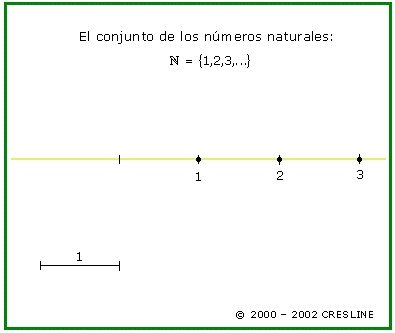
\includegraphics[width=4.1425in,height=3.4964in,keepaspectratio]{img/num1.png}
\par\smallskip
  \textbf{Figura 1}
\end{center}
Ara, sobre la mateixa recta, en la figura 2 hem representat
alguns nombres enters\footnote{%
Recorda que el conjunt dels nombres enters es simbolitza per $%
\mathbb{Z}$ i que $\mathbb{Z}=\{...,-2,-1,0,1,2,...\}$, indicant amb aquesta
notació que $\mathbb{Z}$ és un conjunt els elements del qual són $%
...,-2,-1,0,1,2,...$.}. 
\begin{center}
  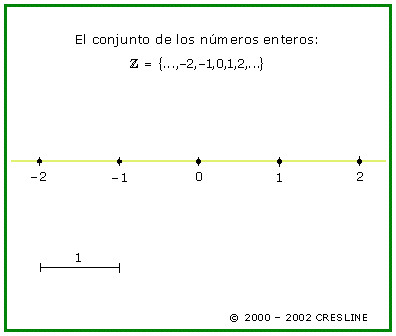
\includegraphics[width=4.1528in,height=3.5276in,keepaspectratio]{img/num2.png}
\par\smallskip
  \textbf{Figura 2%
}
\end{center}
Com hauràs observat tot d’una,
en representar aquests nombres hem hagut d’assenyalar el punt que
correspon a $0$ i els punts que corresponen als nombres
negatius; els punts que corresponen als nombres positius ja
estaven assenyalats en representar els nombres naturals. Per aquesta raó, tenim que $\mathbb{N}\subset \mathbb{Z}$\footnote{%
Amb aquesta notació indiquem que el conjunt $\mathbb{N}$ és un
subconjunt del conjunt $\mathbb{Z}$, és a dir, que tot nombre natural
és un nombre enter.} i $\mathbb{Z}=\mathbb{Z}^{-}\cup \{0\}\cup \mathbb{%
Z}^{+}$\footnote{%
Amb aquesta notació indiquem que qualsevol nombre enter és un nombre enter positiu, és a dir, un nombre natural, o bé és un nombre enter negatiu o bé és zero. En efecte, $\mathbb{Z}^{+}=\mathbb{N}%
=\{1,2,3,...\}$ i $\mathbb{Z}^{-}=\{-1,-2,-3,...\}$ i, per tant, $\mathbb{Z}%
=\mathbb{Z}^{-}\cup \{0\}\cup \mathbb{Z}^{+}$, on $\cup$ és l’operació
entre conjunts que anomenem unió.}. Ara, de nou sobre la mateixa
recta, en la figura 3 hem representat alguns nombres racionals%
\footnote{%
Recorda que el conjunt dels nombres racionals es simbolitza per $%
\mathbb{Q}$ i que 
\begin{equation*}
\mathbb{Q}=\{\frac{n}{m}:n,m\in \mathbb{Z}\text{ i }m\neq 0\}
\end{equation*}%
indicant amb aquesta notació que $\mathbb{Q}$ és un conjunt els elements del qual
són, per exemple, \thinspace $-2,-\frac{1}{3}$ o $\frac{3}{2}$.}.%

\begin{center}
  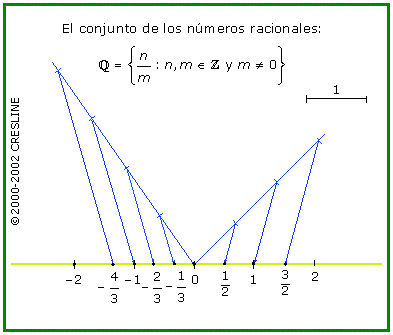
\includegraphics[width=4.1217in,height=3.5172in,keepaspectratio]{img/num3.png}
\par\smallskip
  \textbf{Figura 3}
\end{center}
Com hauràs observat tot d’una, en representar aquests nombres hem hagut d’assenyalar els punts de la recta que corresponen
a les fraccions; els punts que corresponen als nombres
enters\footnote{%
Fraccions equivalents de la forma $\frac{n}{1}$ amb $n\in \mathbb{Z}$} ja
estaven assenyalats. Per aquesta raó, tenim que%
\begin{equation*}
\mathbb{N}\subset \mathbb{Z}\subset \mathbb{Q}
\end{equation*}%
És clar que també tenim en aquest cas que%
\begin{equation*}
\mathbb{Q}=\mathbb{Q}^{-}\cup \{0\}\cup \mathbb{Q}^{+}
\end{equation*}%
és a dir, qualsevol nombre racional és un nombre racional positiu o
bé negatiu o bé és zero.

Arribats a aquest punt, és natural fer-se ara la següent pregunta: una
vegada representats tots els nombres racionals sobre la recta, 
queden buits damunt seu? És a dir,%
hi ha punts de la recta que no corresponen amb cap nombre
considerat fins ara? Per respondre aquesta qüestió, farem la
següent construcció amb regla, escaire i compàs. En la figura 4
hem construït un quadrat de costat $1$ mitjançant regla i escaire.
\begin{center}
  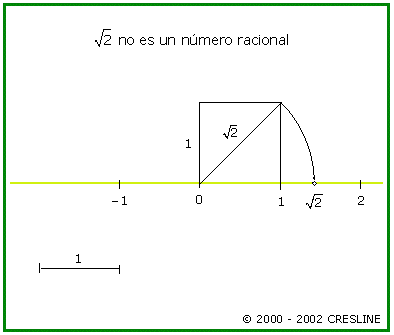
\includegraphics[width=4.1321in,height=3.5172in,keepaspectratio]{img/num4.png}
\par\smallskip
  \textbf{Figura 4}
\end{center}
Pel teorema de Pitàgores\footnote{%
Recorda que el teorema de Pitàgores afirma que un triangle és rectangle si i només si es compleix que%
\begin{equation*}
h^{2}=c_{1}^{2}+c_{2}^{2}
\end{equation*}%
on $h$ indica el costat de major longitud i $c_{1},c_{2}$ els
altres dos costats.}, la diagonal d’aquest quadrat mesura $\sqrt{2}$. Ara,
mitjançant el compàs, hem assenyalat $\sqrt{2}$ sobre la recta.
És $\sqrt{2}$ un nombre racional? Si ho fos, s’hauria de
poder escriure com una fracció%
\begin{equation}
\sqrt{2}=\frac{n}{m}  \label{eq:sqrt2-fraccio}
\end{equation}%
on $n,m\in \mathbb{Z}$. Suposem que és així i veurem que això condueix a una
contradicció\footnote{Volem demostrar que $\sqrt{2}$ no és un nombre racional i,
per fer-ho, utilitzarem el mètode de demostració anomenat reducció a l’absurd:
si a partir de la hipòtesi contrària i de raonaments correctes s’arriba a una
contradicció, necessàriament la conclusió inicial és vertadera.}. Podem suposar
també que la fracció és irreductible, ja que, en cas contrari, la podríem
simplificar fins a obtenir-ne una d’equivalent i irreductible. Aleshores, els
nombres enters $n$ i $m$ són primers entre si i, a més, $m$ no pot ser $1$, ja
que, si ho fos, $\sqrt{2}$ seria un nombre enter; però la construcció anterior
mostra que $\sqrt{2}$ és major que $1$ i menor que $2$. Per tant, es complirà
(\ref{eq:sqrt2-fraccio}) si el quadrat del nombre $\frac{n}{m}$ és $2$, és a dir,%
\begin{equation*}
\left( \frac{n}{m}\right) ^{2}=\frac{n^{2}}{m^{2}}=2.
\end{equation*}%
Ara bé, això no és possible, ja que els nombres enters $n^{2}$ i $m^{2}$,
com que són quadrats, tenen descomposicions en factors primers en què tots els
exponents són parells. A més, com que hem suposat que $n$ i $m$ són primers
entre si, no tenen cap factor en comú. Per tant, la fracció $\frac{n^{2}}{m^{2}}$
també és irreductible i no pot ser igual a$2$.

En definitiva, obtenim una conclusió clara: $\sqrt{2}$ no és cap nombre
racional. Així, en representar tots els nombres racionals sobre la recta,
encara hi queden punts que no corresponen a cap nombre racional; un d’aquests
punts és $\sqrt{2}$. El teorema de Pitàgores permet situar sobre la recta
longituds expressades amb arrels quadrades; per exemple, en la figura 5 hem
situat $\sqrt{3}$ a partir de $\sqrt{2}$,
\begin{center}
  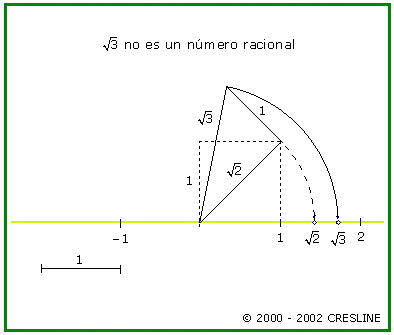
\includegraphics[width=4.1321in,height=3.5163in,keepaspectratio]{img/num5.png}
\par\smallskip
  \textbf{Figura 5}
\end{center}
i de la mateixa manera es poden situar
$\sqrt{5},\sqrt{6},...$ El fet que sigui possible dibuixar sobre una recta
longituds que no estan representades per nombres racionals suggereix
l’existència de nous nombres. A aquests nombres que no són racionals els
anomenarem \textbf{nombres irracionals}.

Tot seguit se’ns planteja una nova pregunta: quina mena de
nombres són els nombres irracionals? La resposta a aquesta qüestió la trobarem
en l’apartat següent.

\subsection{Expressió decimal dels nombres irracionals}

El nombre irracional $\sqrt{2}$ que hem descobert a l’apartat
anterior pot situar-se sobre la recta fent ús del regle i el compàs, com hem vist en la figura 4, però què
classe de nombre és? Serà un nombre que, elevat al quadrat, sigui 
$2$. Per construcció, sabem que $\sqrt{2}$ està entre $1$ i $2$.
Continuem provant valors de $\sqrt{2}$, per tempteig, usant una calculadora
per trobar $1.1^{2},1.2^{2}$, etc. (de moment, no val fer servir la tecla $%
\sqrt{}$). Després de diverses proves, obtindrem els següents
resultats:

\begin{enumerate}
\item $\sqrt{2}$ està comprès entre $1.4$ i $1.5$ ja que $%
1.4^{2}=1.96$ i $1.5^{2}=2.25$

\item $\sqrt{2}$ està comprès entre $1.41$ i $1.42$ ja que $%
1.41^{2}=1.9881$ i $1.42^{2}=2.0164$

\item $\sqrt{2}$ està comprès entre $1.414$ i $1.415$ ja que $%
1.414^{2}=1.999396$ i $1.415^{2}=2.002225$
\end{enumerate}

Encara no hem trobat un nombre decimal el quadrat del qual sigui $2$, però
hem millorat el resultat que havíem obtingut per construcció.
Aquest mètode permetrà assolir la precisió que es vulgui amb
només repetir aquest procés tantes vegades com sigui necessari. Naturalment, la
calculadora té la tecla $\sqrt{}$ per calcular arrels. Fent-la servir, obtindràs un resultat com el següent (depèn de quantes
xifres sigui capaç de manejar la calculadora)%
\begin{equation*}
\sqrt{2}=1.414213562
\end{equation*}%
però, com pots imaginar en seguida, aquest resultat no és exacte, perquè
si ho fos, aleshores $\sqrt{2}$ seria un nombre racional i això no
és possible com s’ha vist a l’apartat anterior. A més, per la
mateixa raó, $\sqrt{2}$ tampoc és un nombre decimal periòdic%
\footnote{%
Recorda que tot nombre decimal exacte o periòdic admet una fracció generatriu que el representa i, per tant, és un nombre racional.}%
. Per tant, només podem escriure%
\begin{equation*}
\sqrt{2}=1.41421356...
\end{equation*}%
i, de la mateixa manera, passa que%
\begin{equation*}
\sqrt{3}=1.732050808...
\end{equation*}%
i, en general, tots els nombres que hem anomenat irracionals
tenen una expressió decimal que té un nombre infinit de xifres
decimals no periòdiques. Aquesta caracterització dels nombres
irracionals condueix a la definició de nombre real com veurem en
el següent apartat.

\subsection{El conjunt dels nombres reals}

Dels dos apartats anteriors podem concloure afirmant que no tots els nombres decimals que necessitem per resoldre problemes elementals de
mesura de longituds són finits o periòdics, és a dir, no són nombres racionals. Aquesta insuficiència del conjunt $\mathbb{Q}$ condueix a la
necessitat d’ampliar-lo amb els nombres decimals infinits no periòdics, és a dir, amb els nombres irracionals. D’aquesta manera, formem un
nou conjunt de nombres que anomenarem \textbf{conjunt dels nombres reals} i que simbolitzarem per $\mathbb{R}$. Per tant, un nombre real serà un nombre decimal exacte, periòdic o no. És
clar que si simbolitzem el conjunt dels nombres irracionals per $%
\mathbb{I}$, aleshores%
\begin{equation*}
\mathbb{R}=\mathbb{Q}\cup \mathbb{I}
\end{equation*}%
i, per tant, és evident que per construcció es compleix%
\begin{equation*}
\mathbb{N}\subset \mathbb{Z}\subset \mathbb{Q}\subset \mathbb{R}
\end{equation*}%
El conjunt dels nombres reals $\mathbb{R}$ conté, a més de $%
0 $, els nombres decimals positius (situats a la seva dreta en la recta)
i els negatius (situats a la seva esquerra en la recta). Si simbolitzem per $%
\mathbb{R}^{+}$ el conjunt dels nombres decimals positius i per $%
\mathbb{R}^{-}$, el dels negatius, obtenim%
\begin{equation*}
\mathbb{R}=\mathbb{R}^{-}\cup \{0\}\cup \mathbb{R}^{+}
\end{equation*}%
i els tres conjunts són disjunts entre si\footnote{%
Recorda que dos conjunts $A$ i $B$ s’anomenen disjunts si el seu intersecció és el conjunt buit $A\cap B=\varnothing $.}. Com a resum, en
la figura 6 mostrem la classificació dels nombres reals.
\begin{center}
  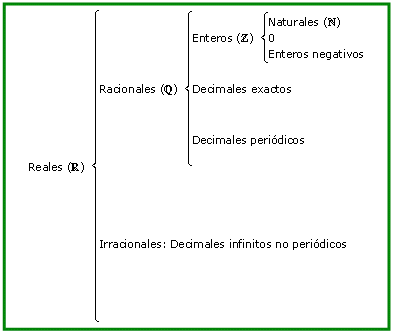
\includegraphics[width=4.1217in,height=3.4964in,keepaspectratio]{img/num11.png}
\par\smallskip
  \textbf{Figura 6}
\end{center}


Finalment, ens queda per resoldre una última qüestió molt
important. Situats tots els nombres reals sobre la recta considerada
a l’apartat 1, queda aquesta recta sense cap forat?
La resposta a aquesta pregunta és afirmativa com veurem en el següent
apartat.

\subsection{La recta real}

El problema que ens plantegem ara és el següent: donat un nombre
real, podem identificar-lo com un únic punt de la
recta considerada a l’apartat 1? i, recíprocament, donat un punt de
la recta, podem identificar-lo com un únic nombre real? Com veurem a continuació, la resposta és sí a ambdues
preguntes. D’aquesta manera, s’estableix una correspondència bijectiva entre
els nombres reals i els punts de la recta i, com a conseqüència, els nombres reals omplen totalment la recta. D’aquí ve el nom de
recta real a la recta com representació gràfica del conjunt dels
nombres reals.

\subsubsection{Tot nombre real és un punt de la recta}

Si el nombre real és un nombre racional ja sabem que podem
situar-lo com un únic punt de la recta; hem representat alguns nombres racionals en la figura 3. Si el nombre és irracional, també hem vist com es situa sobre la recta en els casos més
senzills com $\sqrt{2}$ o $\sqrt{3}$; hem situat aquests punts en les
figures 4 i 5, respectivament. Ara bé, hi ha altres nombres
irracionals que no admeten construccions geomètriques tan simples
(fent servir regle i compàs). Per exemple, la longitud d’una circumferència%
\footnote{%
Recorda que la longitud $L$ d’una circumferència de radi $r$ ve donada
per la fórmula $L=2\pi r$.} de diàmetre $1$ és el nombre pi 
\begin{equation*}
\pi =3.141592654...
\end{equation*}%
que també és un nombre irracional. Podem aproximar $\pi$ de la
següent manera: en la circumferència de diàmetre $1$ s’inscriu i
es circumscriu un hexàgon regular. La longitud d’aquesta circumferència serà menor que el perímetre\footnote{%
Recorda que s’anomena perímetre d’un polígon a la suma de tots
els seus costats.} del hexàgon circumscrit i major que el perímetre del hexàgon inscrit. En la mateixa circumferència es van inscrivint i
circumscrivint successivament polígons regulares amb doble nombre
de costats que el polígon anterior i es van calculant els perímetres respectius. D’aquesta manera, es pot aproximar $\pi$ tant com es
vulgui. En la figura 7 hem anotat algunes aproximacions successives de $%
\pi $.
\begin{center}
  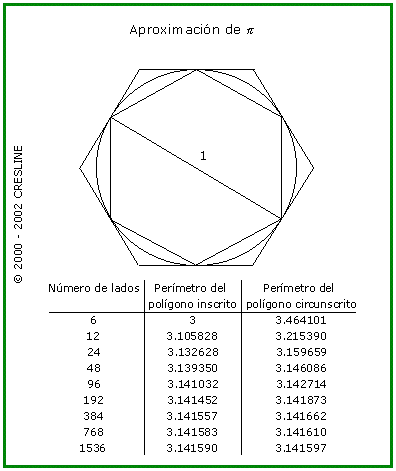
\includegraphics[width=4.1528in,height=4.9338in,keepaspectratio]{img/num8.png}
\par\smallskip
  \textbf{Figura 7}
\end{center}
En general, ja que, el problema es redueix a situar sobre la recta un
nombre decimal infinit no periòdic. Per veure com es fa
això, utilitzarem el nombre irracional $\sqrt{2}$ que hem construït
mitjançant regla i compàs a l’apartat 1. Mitjançant calculadora,
obtenim la seva expressió decimal%
\begin{equation*}
\sqrt{2}=1.41421356...
\end{equation*}%
A partir del nombre decimal podem construir la següent successió
de nombres racionals%
\begin{equation}
1,1.4,1.41,1.414,1.4142,1.41421,...  \label{eq:sqrt2-defecte}
\end{equation}%
obtinguts prenent les primeres xifres decimals del nombre. Cada nombre d’aquesta llista és menor que $\sqrt{2}$ i es diu que són les \textbf{%
aproximacions successives per defecte} de $\sqrt{2}$. Sumant ara una
unitat a l’última xifra decimal dels nombres que apareixen en (\ref{eq:sqrt2-defecte}), obtenim%
\begin{equation}
2,1.5,1.42,1.415,1.4143,1.41422,...  \label{eq:sqrt2-exces}
\end{equation}%
Tots aquests nombres racionals són majors que $\sqrt{2}$ i es diu que
són les \textbf{aproximacions successives per excés} de $\sqrt{2}$. Per
tant, el punt de la recta que hem d’assignar a$\sqrt{2}$ s’ha de situar
una mica més a la dreta que els punts corresponents als nombres racionals en (\ref{eq:sqrt2-defecte}) i una mica més a l’esquerra que els
corresponents a (\ref{eq:sqrt2-exces}). En la figura 8, hem situat sobre la recta
els nombres racionals de (\ref{eq:sqrt2-defecte}) i (\ref{eq:sqrt2-exces}).
\begin{center}
  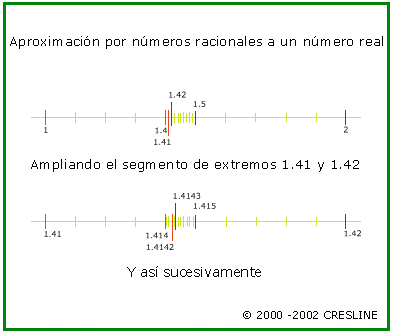
\includegraphics[width=4.1217in,height=3.5068in,keepaspectratio]{img/num6.png}
\par\smallskip
  \textbf{Figura 8}
\end{center}
Si ara
considerem els segments sobre la recta d’extrems $1$ i $2$, $1.4$ i $%
1.5 $, $1.41$ i $1.42\,$, ... tenim que les seves longituds són respectivament 
$1$, $0.1$, $0.01$, ... Els segments sobre la recta s’anomenen \textbf{%
intervals} i es denoten col·locant els extrems entre parèntesis
quadrats, és a dir, els segments de recta considerats anteriorment s’escriuen així%
\begin{equation}
\lbrack 1,2],[1.4,1.5],[1.41,1.42],...  \label{eq:sqrt2-intervals}
\end{equation}%
Hem dibuixat aquests segments en la figura 9, i ens adonem en
seguida que cada interval està contingut en l’anterior. Diem
aleshores que són \textbf{intervals encaixats}. 
\begin{center}
  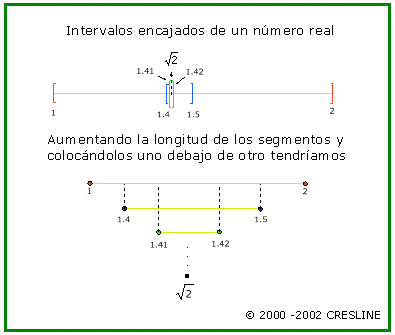
\includegraphics[width=4.1425in,height=3.5068in,keepaspectratio]{img/num7.png}
\par\smallskip
  \textbf{Figura 9}
\end{center}
Ara
hem d’assumir\footnote{%
Aquest resultat encara que és intuïtiu, és una de les propietats fonamentals
que es dedueixen de la construcció axiomàtica dels nombres
reals que es veurà en estudis superiors de matemàtiques.} un
resultat teòric conegut com \textbf{propietat dels intervals
encaixats}\footnote{%
Segons aquesta propietat, en tota successió d’intervals encaixats tals
que la seva longitud es fa tan petita com es vulgui existeix un únic
punt pertanyent a tots els intervals de la successió.}. Segons
aquesta propietat, tots aquests intervals tenen un únic punt en comú; de
fet hi ha infinits, ja que, hi ha infinites xifres decimals en l’expressió
decimal de $\sqrt{2}$, i la longitud de cada un d’ells és la desena
part de l’anterior. Com que, per construcció, tots els intervals (%
\ref{eq:sqrt2-intervals}) contenen $\sqrt{2}$, aquest punt comú correspon a$\sqrt{2}$%
. Es diu aleshores que la \textbf{successió d’intervals encaixats }(\ref{eq:sqrt2-intervals})\textbf{\ define} $\sqrt{2}$; encara que és impossible trobar el punt
corresponent a $\sqrt{2}$, tanmateix, la propietat dels intervals
encaixats n’assegura l’existència sobre la recta. A partir d’aquesta definició, es comprèn per què els nombres racionals i els
irracionals estan tan pròxims uns dels altres fins al punt que
entre dos nombres reals qualssevol existeixen infinits racionals i
infinits irracionals.

\subsubsection{Tot punt de la recta és un nombre real}

Si en una recta s’han fixat un origen i una unitat, tot punt $P$ d’aquesta
recta correspon a un únic nombre real. El procés que cal seguir per identificar $P$ com un nombre real és invers al
seguit a l’apartat anterior. En la figura 10 hem situat un punt
qualsevol $P$ de la recta.
\begin{center}
  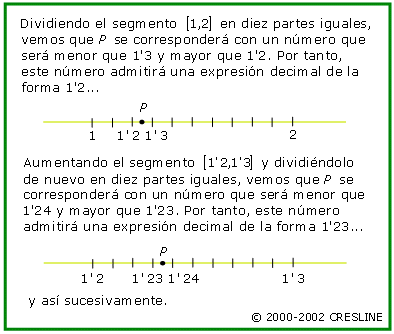
\includegraphics[width=4.1321in,height=3.5068in,keepaspectratio]{img/num9.png}
\par\smallskip
  \textbf{Figura 10}
\end{center}
En teoria, el procés indicat en
la figura anterior es pot repetir indefinidament. A més, com tots
els intervals que anem construint són encaixats i la longitud de cada
un d’ells és la desena part de l’anterior, per la propietat dels
intervals encaixats, existirà un nombre real i només un comú a tots ells i aquest nombre real correspondrà per
construcció al punt $P$. Tanmateix, hem de fer una important
observació. La possible expressió decimal del nombre real
corresponent a $P$ serà única excepte quan $P$ coincida amb
alguna de les subdivisions successives. En efecte, si en un pas del procés
de subdivisió, $P$ s’identifica amb un nombre de la subdivisió realitzada en aquest pas, en el pas següent tenim dos possibles
eleccions: una consisteix a triar el subinterval a l’esquerra de $P$, i
l’altra, consisteix a triar el subinterval a la dreta de $P$. En la
figura 11 es mostra amb més de detall en tractar un exemple. 
\begin{center}
  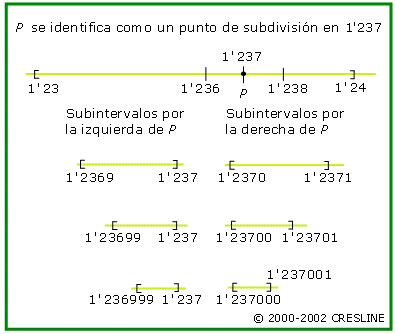
\includegraphics[width=4.1321in,height=3.5163in,keepaspectratio]{img/num10.png}
\par\smallskip
  \textbf{Figura 11}
\end{center}
Ens adonem en seguida que l’expressió decimal del nombre real corresponent a $P$ per l’esquerra serà de la forma $%
1.236999...$, mentre que la seva expressió decimal per la dreta serà $%
1.237000...$. Sabem que cadascuna d’aquestes col·leccions d’intervals
encaixats ha de tenir un únic nombre real comú i podem
observar que en cada col·lecció el nombre decimal exacte $1.237$,
corresponent al punt $P$, pertany a tots els intervals. Per tant,
les dues successions d’intervals encaixats defineixen el mateix nombre $%
1.237$ i aquest és el que correspon al punt $P$. Com a conseqüència, $%
1.236999...$ i $1.237000...$ representen el mateix nombre real (racional) 
$1.237$.

En resum, tot punt de la recta està representat per un nombre
amb, possiblement, infinites xifres decimals, però identificant els
decimals exactes amb els decimals de període 9 i amb els de període 0.

En aquesta recta, entre dos racionals existeix sempre un altre racional, entre dos
irracionals existeix sempre un racional tan proper com es
vulgui. Aquesta idea prové de la forma com s’han definit els nombres
irracionals a partir dels intervals encaixats d’extrems racionals.

\section{Operacions amb nombres reals}

En aquesta secció veurem que tot el treball operatiu amb nombres
reals s’ha de fer amb aproximacions; per sumar i multiplicar dos nombres reals caldrà sumar i multiplicar les seves aproximacions. També
es poden fer les operacions geomètricament, utilitzant les
operacions amb segments. Admetrem que les operacions anteriors en $%
\mathbb{R}$ compleixen les mateixes propietats que en $\mathbb{Q}$. D’aquesta
manera, el conjunt dels nombres reals té estructura de cos. Com a
conseqüència, podrem aplicar totes les propietats que es dedueixen d’aquesta
estructura algebraica a $\mathbb{R}$; per exemple, podrem resoldre
equacions com%
\begin{equation*}
2x+3=4
\end{equation*}%
de la següent manera%
\begin{equation*}
2x=4+(-3)
\end{equation*}%
ja que l’equació $x+a=b$ té la solució única $x=b+(-a)$;
efectuant operacions, tenim%
\begin{equation*}
2x=1
\end{equation*}%
Aleshores,%
\begin{equation*}
x=\frac{1}{2}
\end{equation*}%
ja que l’equació $a\cdot x=b$, amb $a\neq 0$, té la solució 
única $x=\frac{1}{a}\cdot b$.

\subsection{Aproximacions}

En la pràctica, en treballar amb els nombres reals que són
irracionals ens trobem amb el problema de saber com cal
escriure’ls i operar amb ells. En no poder-los escriure de forma exacta, ja
que són nombres amb infinites xifres decimals, ens veiem obligats a
treballar amb aproximacions. Les aproximacions decimals per defecte i per
excés de cada grau, utilitzades per identificar un nombre irracional
sobre la recta real, ens donen un bon mètode d’aproximació.
\begin{center}
  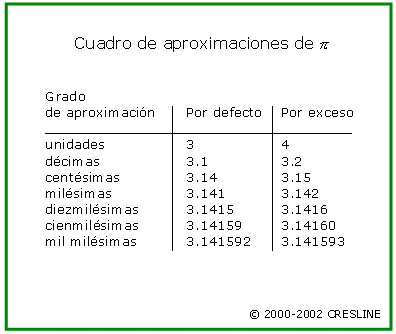
\includegraphics[width=4.1528in,height=3.5068in,keepaspectratio]{img/num12.png}
\end{center}


És clar que treballar amb una aproximació, en lloc de treballar amb el
valor exacte, comporta una certa càrrega d’error. Tot i que aquí no
tractarem el problema dels errors en els càlculs amb nombres
aproximats, en els resultats de les operacions amb nombres reals
sempre precisarem les xifres significatives que podem considerar
correctes; a l’apartat següent ho veurem amb alguns exemples.

\subsection{Suma i producte de nombres reals}

Com ja sabem com se sumen i es multipliquen dos nombres racionals
(encara que dependrà de com estiguin representats els dos nombres, podrem fer-ho sempre de forma exacta utilitzant fraccions), només caldrà tractar els dos casos següents: suma i producte de
dos nombres irracionals, i suma i producte de dos nombres, un
racional i l’altre irracional.

\subsubsection{Suma}

Per sumar dos nombres irracionals, en no poder-los escriure de forma
exacta, ens veiem obligats a treballar amb les seves aproximacions. Per exemple,
per sumar $\sqrt{2}$ i $\pi $, primer considerem les seves aproximacions
decimals per defecte i per excés:%
\begin{equation*}
\begin{array}{cc}
\sqrt{2} & \left\{ 
\begin{array}{cccccc}
1 & 1.4 & 1.41 & 1.414 & 1.4142 & \cdots \\ 
2 & 1.5 & 1.42 & 1.415 & 1.4143 & \cdots%
\end{array}%
\right.%
\end{array}%
\end{equation*}%
i%
\begin{equation*}
\begin{array}{cc}
\pi & \left\{ 
\begin{array}{cccccc}
3 & 3.1 & 3.14 & 3.141 & 3.1415 & \cdots \\ 
4 & 3.2 & 3.15 & 3.142 & 3.1416 & \cdots%
\end{array}%
\right.%
\end{array}%
\end{equation*}%
Després, sumem cada aproximació per defecte (resp. per excés) de 
$\sqrt{2}$ amb la corresponent aproximació per defecte (resp. per
excés) del mateix grau de $\pi $, obtenint les següents aproximacions
de $\sqrt{2}+\pi $:%
\begin{equation*}
\begin{array}{cc}
\sqrt{2}+\pi & \left\{ 
\begin{array}{cccccc}
4 & 4.5 & 4.55 & 4.555 & 4.5557 & \cdots \\ 
6 & 4.7 & 4.57 & 4.557 & 4.5559 & \cdots%
\end{array}%
\right.%
\end{array}%
\end{equation*}%
Finalment, a partir d’aquestes aproximacions, determinem quantes
xifres podem considerar com correctes. En aquest cas, podem assegurar
quatre xifres correctes en el resultat%
\begin{equation*}
\sqrt{2}+\pi =4.555...
\end{equation*}%
És clar que, procedint d’aquesta manera, podem trobar tantes xifres
decimals exactes com vulguem, n’hi haurà prou amb augmentar la precisió
dels sumands (ampliar el nombre d’aproximacions decimals).

En general, si volem obtenir la suma (o la resta) amb un cert grau $n$
d’aproximació, les aproximacions dels sumands s’hauran de prendre
amb aproximació de grau $n+1$; per exemple, si volem calcular $%
\sqrt{2}+\pi$ amb aproximació fins a les mil·lèsimes, s’han de prendre $%
\sqrt{2}$ i $\pi$ amb aproximació fins a les deu mil·lèsimes, és
a dir, $\sqrt{2}=1.4142...$ i $\pi =3.1415...$ i, d’aquesta manera, obtenim 
\begin{equation*}
\sqrt{2}+\pi =4.555\overset{?}{7}...=4.555...
\end{equation*}%
assegurant la precisió buscada.

Per sumar dos nombres, un racional i l’altre irracional, es procedeix
de la mateixa manera. Per exemple, per sumar $7/6$ i $\sqrt{2}$, primer donarem
l’expressió decimal del nombre racional%
\begin{equation*}
\frac{7}{6}=1.1666...
\end{equation*}%
i després considerarem les seves aproximacions decimals per defecte i per
excés%
\begin{equation*}
\begin{array}{cc}
\frac{7}{6} & \left\{ 
\begin{array}{cccccc}
1 & 1.1 & 1.16 & 1.166 & 1.1666 & \cdots \\ 
2 & 1.2 & 1.17 & 1.167 & 1.1667 & \cdots%
\end{array}%
\right.%
\end{array}%
\end{equation*}%
De la mateixa manera, tenim%
\begin{equation*}
\begin{array}{cc}
\sqrt{2} & \left\{ 
\begin{array}{cccccc}
1 & 1.4 & 1.41 & 1.414 & 1.4142 & \cdots \\ 
2 & 1.5 & 1.42 & 1.415 & 1.4143 & \cdots%
\end{array}%
\right.%
\end{array}%
\end{equation*}%
Per tant,%
\begin{equation*}
\begin{array}{cc}
\frac{7}{6}+\sqrt{2} & \left\{ 
\begin{array}{cccccc}
2 & 2.5 & 2.57 & 2.580 & 2.5808 & \cdots \\ 
4 & 2.7 & 2.59 & 2.582 & 2.5810 & \cdots%
\end{array}%
\right.%
\end{array}%
\end{equation*}%
i, en conseqüència,%
\begin{equation*}
\frac{7}{6}+\sqrt{2}=2.58...
\end{equation*}%
és a dir, només podem assegurar dues xifres decimals exactes en el
resultat.

\subsubsection{Producte}

De la mateixa manera a com hem fet la suma, es fa producte. Per exemple,
per multiplicar $\sqrt{2}$ i $\pi$ considerem les seves respectives
aproximacions decimals per defecte i per excés%
\begin{equation*}
\begin{array}{cc}
\sqrt{2} & \left\{ 
\begin{array}{cccccc}
1 & 1.4 & 1.41 & 1.414 & 1.4142 & \cdots \\ 
2 & 1.5 & 1.42 & 1.415 & 1.4143 & \cdots%
\end{array}%
\right.%
\end{array}%
\end{equation*}%
i%
\begin{equation*}
\begin{array}{cc}
\pi & \left\{ 
\begin{array}{cccccc}
3 & 3.1 & 3.14 & 3.141 & 3.1415 & \cdots \\ 
4 & 3.2 & 3.15 & 3.142 & 3.1416 & \cdots%
\end{array}%
\right.%
\end{array}%
\end{equation*}%
Després, multipliquem cada aproximació per defecte (resp. per excés) de 
$\sqrt{2}$ per la corresponent aproximació per defecte (resp. per
excés) del mateix grau de $\pi $, obtenint%
\begin{equation*}
\begin{array}{cc}
\sqrt{2}\cdot \pi & \left\{ 
\begin{array}{cccccc}
3 & 4.34 & 4.4274 & 4.441374 & 4.44270930 & \cdots \\ 
8 & 4.80 & 4.4730 & 4.445930 & 4.44316488 & \cdots%
\end{array}%
\right.%
\end{array}%
\end{equation*}%
Finalment, a partir d’aquestes aproximacions, determinem quantes
xifres podem considerar com correctes. En aquest cas, podem assegurar
tres xifres correctes en el resultat%
\begin{equation*}
\sqrt{2}\cdot \pi =4.44...
\end{equation*}%
És clar que, procedint d’aquesta manera, podem trobar tantes xifres
decimals exactes com vulguem; n’hi haurà prou amb augmentar la precisió
dels factors (ampliar el nombre d’aproximacions decimals).

En general, si volem obtenir el producte (o el quocient) amb $n$ xifres
significatives\footnote{%
Recorda que si $b$ és una aproximació d’un nombre real $a$, les
xifres significatives de $b$ són aquelles que coincideixen amb les de $a$,
excepte els zeros que tenen com a única finalitat sigui situar la coma decimal},
haurem de prendre una xifra significativa més per als factors; per
exemple, en trobar-se $\sqrt{2}\cdot \pi$ entre $3$ i $8$, per obtenir
un resultat amb aproximació fins a les centèsimes, necessitem
garantir que tres de les seves xifres siguin significatives, i, per tant,
haurem de prendre cada factor amb quatre xifres significatives, és a dir, $%
\sqrt{2}=1.4142...$ i $\pi =3.1415...$ i, d’aquesta manera, obtenim%
\begin{equation*}
\sqrt{2}\cdot \pi =4.44\overset{?}{\overbrace{27093}}...=4.44...
\end{equation*}

\subsubsection{Operacions amb segments}

Per sumar (o restar) dos nombres reals $a$ i $b$, el punt que
correspon al nombre $a+b$ s’obté traslladant el punt
corresponent al nombre $a$ una distància igual a la longitud del
segment corresponent al nombre $b$ cap a la dreta, si $b$ es
positiu, i cap a l’esquerra, si $b$ és negatiu; en la figura 12,
suposant que $a$ i $b$ són positius, es mostra la suma $a+b$ i la resta 
$a-b=a+(-b)$. 
\begin{center}
  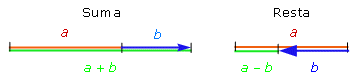
\includegraphics[width=3.7455in,height=0.8622in,keepaspectratio]{img/num33.png}
\par\smallskip
  \textbf{Figura 12}
\end{center}
Per exemple, a la figura següent,
utilitzant procediments geomètrics, representem sobre la recta real 
$\sqrt{13}-\sqrt{2}$.
\begin{center}
  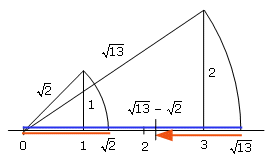
\includegraphics[width=2.84in,height=1.6725in,keepaspectratio]{img/num36.png}
\end{center}


Per obtenir gràficament el producte de dos nombres reals $a$ i $b$%
, aplicarem el teorema de Thales\footnote{%
Recorda que el teorema de Thales diu que els segments determinats sobre
dues rectes concurrents tallades per diverses rectes paral·leles són
proporcionals.}: suposem que hem situat sobre la recta real els nombres $a$ i $b$, tracemos una recta auxiliar pel punt $O$
corresponent al nombre $0$ i, mitjançant el compàs, construïm
damunt seu i a partir de $O$ un segment de longitud $b$, obtindrem de
aquest manera un punt $P$. Unimos ara amb una recta el punt $P$ amb el punt 
$U$ corresponent al nombre $1$. Mitjançant regla i escaire, tracem
pel punt corresponent a $b$ una recta paral·lela a la recta anterior
que tallarà a la recta auxiliar en un punt $Q$. Mitjançant compàs,
construimos sobre la recta real un segment de longitud $OQ$, la longitud de
aquest segment serà el producte $a\cdot b$; en la figura 13 es mostral
mètode seguit per obtenir gràficamente $a\cdot b$.
\begin{center}
  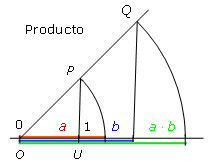
\includegraphics[width=2.2157in,height=1.7244in,keepaspectratio]{img/num34.png}
\par\smallskip
  \textbf{Figura 13}
\end{center}
Observa que, pel teorema de Thales,%
\begin{equation*}
\frac{\overline{OP}}{\overline{OU}}=\frac{\overline{OQ}}{b}
\end{equation*}%
però $\overline{OP}=a$ i $\overline{OU}=1$, per tant%
\begin{equation*}
\overline{OQ}=a\cdot b
\end{equation*}%
Per exemple, a la figura següent, utilitzant procediments geomètrics, representem sobre la recta real $\sqrt{13}\cdot \sqrt{2}$.
\begin{center}
  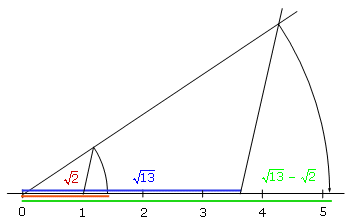
\includegraphics[width=3.6633in,height=2.3298in,keepaspectratio]{img/num37.png}
\end{center}


Per obtenir gràficament el invers d’un nombre real $a$, amb $%
a\neq 0$, podem aplicar la mateixa construcció anterior però prenent
ara$b=1$; en la figura 14 podràs veure els passos que cal fer per
obtenir $1/a$. 
\begin{center}
  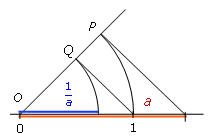
\includegraphics[width=2.2355in,height=1.4538in,keepaspectratio]{img/num35.png}
\par\smallskip
  \textbf{Figura 14}
\end{center}
Observa que, pel teorema de Thales,%
\begin{equation*}
\frac{\overline{OP}}{a}=\frac{\overline{OQ}}{1}
\end{equation*}%
però $\overline{OP}=1$, per tant%
\begin{equation*}
\overline{OQ}=\frac{1}{a}
\end{equation*}%
Finalment, per obtenir gràficamente el quocient $\frac{a}{b}$ de dos nombres reals $a$ i $b$, amb $b\neq 0$, primer es representarà el
invers de $b$ i, després, s’obtindrà el producte $a\cdot \frac{1}{b%
}$. Per exemple, a la figura següent, utilitzant procediments geomètrics, representem sobre la recta real $\frac{\sqrt{13}}{\sqrt{2}}$.%

\begin{center}
  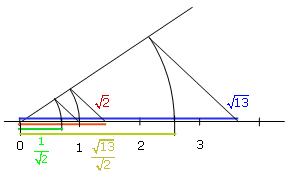
\includegraphics[width=3.0485in,height=1.8611in,keepaspectratio]{img/num38.png}
\end{center}


\subsection{El cos dels nombres reals}

Es demostra (en aquest nivell encara no disposem de les eines
suficients per provar aquests resultats) que les operacions de suma i
producte de nombres reals compleixen les mateixes propietats que la suma i
el producte de nombres racionals.

L’operació suma de nombres reals compleix les següents
propietats:

\begin{enumerate}
\item Llei de composició interna: $a+b\in \mathbb{R}$, per tot $a,b\in 
\mathbb{R}$

\item Associativa: $a+(b+c)=(a+b)+c$, per tot $a,b,c\in \mathbb{R}$

\item Element neutre: existeix $0\in \mathbb{R}$ tal que $a+0=0+a=a$, per
tot $a\in \mathbb{R}$.

\item Commutativa: $a+b=b+a$, per tot $a,b\in \mathbb{R}$

\item Element simètric: per cada $a\in \mathbb{R}$ existeix $-a\in 
\mathbb{R}$, anomenat \textbf{oposat} de $a$, tal que $a+(-a)=(-a)+a=0$
\end{enumerate}

L’operació producte de nombres reals compleix les següents
propietats:

\begin{enumerate}
\item[6.] Llei de composició interna: $a\cdot b\in \mathbb{R}$, per
tot $a,b\in \mathbb{R}$

\item[7.] Associativa: $a\cdot (b\cdot c)=(a\cdot b)\cdot c$, per tot $%
a,b,c\in \mathbb{R}$

\item[8.] Element neutre: existeix $1\in \mathbb{R}$ tal que $a\cdot 1=1\cdot
a=a$, per tot $a\in \mathbb{R}$

\item[9.] Commutativa: $a\cdot b=b\cdot a$, per tot $a,b\in \mathbb{R}$

\item[10.] Element simètric: per cada $a\in \mathbb{R}$ amb $a\neq 0$ existeix $%
1/a\in \mathbb{R}$, anomenat \textbf{invers} de $a$, tal que $a\cdot
(1/a)=(1/a)\cdot a=1$
\end{enumerate}

Finalment, les dues operacions compleixen la propietat

\begin{enumerate}
\item[11.] Distributiva del producte respecte de la suma:%
\begin{equation*}
\begin{array}{c}
a\cdot (b+c)=a\cdot b+a\cdot c \\ 
(b+c)\cdot a=b\cdot a+c\cdot a%
\end{array}%
\end{equation*}%
per a tot $a,b,c\in \mathbb{R}$
\end{enumerate}

Pel fet de satisfàr aquestes 11 propietats es diu que el conjunt $%
\mathbb{R}$ dels nombres reals és un \textbf{cos} o que té la
estructura de cos. Per aquesta raó, es diu que $\mathbb{R}$ és el 
\textbf{cos dels nombres reals}.

És clar que per restar i dividir dos nombres reals procedirem en la
forma habitual, és a dir,%
\begin{equation*}
a-b=a+(-b)
\end{equation*}%
i%
\begin{equation*}
a:b=a\cdot \frac{1}{b}
\end{equation*}%
sempre que $b\neq 0$. Les regles de càlcul en $\mathbb{R}$, que es
dedueixen per tenir estructura de cos, són les mateixes que les del conjunt
dels nombres racionals $\mathbb{Q}$, que també té estructura
de cos. A continuació, considerem algunes d’elles pel seu interès en la pràctica: si $a,b,c\in \mathbb{R}$, aleshores es compleixen les
següents propietats

\begin{enumerate}
\item Si $a+b=b$, aleshores $a=0$
\end{enumerate}

En efecte, 
\begin{align*}
a+b &=b \\
\left( a+b\right) +(-b) &=b+(-b) \\
a+(b+(-b)) &=b+(-b) \\
a+0 &=0 \\
a &=0
\end{align*}

\begin{enumerate}
\item[2.] Si $a\cdot b=b$ i $b\neq 0$, aleshores $a=1$
\end{enumerate}

En efecte,%
\begin{align*}
a\cdot b &=b \\
(a\cdot b)\cdot \frac{1}{b} &=b\cdot \frac{1}{b} \\
a\cdot \left( b\cdot \frac{1}{b}\right) &=b\cdot \frac{1}{b} \\
a\cdot 1 &=1 \\
a &=1
\end{align*}

\begin{enumerate}
\item[3.] Si $a+b=0$, aleshores $a=-b$
\end{enumerate}

En efecte,%
\begin{align*}
a+b &=0 \\
(a+b)+(-b) &=0+(-b) \\
a+(b+(-b)) &=-b \\
a+0 &=-b \\
a &=-b
\end{align*}

\begin{enumerate}
\item[4.] Si $a\cdot b=1$ i $b\neq 0$, aleshores $a=\frac{1}{b}$
\end{enumerate}

En efecte,%
\begin{align*}
a\cdot b &=1 \\
(a\cdot b)\cdot \frac{1}{b} &=1\cdot \frac{1}{b} \\
a\cdot \left( b\cdot \frac{1}{b}\right) &=\frac{1}{b} \\
a\cdot 1 &=\frac{1}{b} \\
a &=\frac{1}{b}
\end{align*}

\begin{enumerate}
\item[5.] Si $a+c=b+c$, aleshores $a=b$
\end{enumerate}

En efecte,%
\begin{align*}
a+c &=b+c \\
(a+c)+(-c) &=(b+c)+(-c) \\
a+(c+(-c)) &=b+(c+(-c)) \\
a+0 &=b+0 \\
a &=b
\end{align*}

\begin{enumerate}
\item[6.] Si $a\cdot c=b\cdot c$ i $c\neq 0$, aleshores $a=b$
\end{enumerate}

En efecte,%
\begin{align*}
a\cdot c &=b\cdot c \\
(a\cdot c)\cdot \frac{1}{c} &=(b\cdot c)\cdot \frac{1}{c}\text{ç} \\
a\cdot \left( c\cdot \frac{1}{c}\right) &=b\cdot \left( c\cdot \frac{1}{c}%
\right) \\
a\cdot 1 &=b\cdot 1 \\
a &=b
\end{align*}

\begin{enumerate}
\item[7.] $a\cdot 0=0$
\end{enumerate}

En efecte,%
\begin{align*}
a+(-a) &=0 \\
a\cdot (1+(-1)) &=0 \\
a\cdot 0 &=0
\end{align*}

\begin{enumerate}
\item[8.] Si $a\cdot b=0$, aleshores $a=0$ o $b=0$
\end{enumerate}

En efecte, si $a\neq 0$ aleshores%
\begin{align*}
a\cdot b &=0 \\
a\cdot b &=a\cdot 0 \\
b\cdot a &=0\cdot a
\end{align*}%
d’on $b=0$ pel apartat anterior. Anàlogament, si $b\neq 0$
aleshores%
\begin{align*}
a\cdot b &=0 \\
a\cdot b &=0\cdot b
\end{align*}%
d’on $a=0$ pel apartat anterior.

\begin{enumerate}
\item[9.] $a\cdot (-b)=(-a)\cdot b=-(a\cdot b)$
\end{enumerate}

En efecte,%
\begin{align*}
a\cdot b+a\cdot (-b) &=a\cdot (b+(-b)) \\
&=a\cdot 0 \\
&=0
\end{align*}%
d’on $a\cdot (-b)=-(a\cdot b)$. Anàlogament,%
\begin{align*}
a\cdot b+(-a)\cdot b &=(a+(-a))\cdot b \\
&=0\cdot b \\
&=b\cdot 0 \\
&=0
\end{align*}

\begin{enumerate}
\item[10.] $(-1)\cdot a=-a$
\end{enumerate}

En efecte,%
\begin{align*}
a+(-1)\cdot a &=(1+(-1))\cdot a \\
&=0\cdot a \\
&=a\cdot 0 \\
&=0
\end{align*}%
Per tant, $(-1)\cdot a=-a$, ja que l’oposat d’un nombre és únic.

\begin{enumerate}
\item[11.] $-(-a)=a$
\end{enumerate}

En efecte,%
\begin{equation*}
(-a)+a=0
\end{equation*}%
per tant, $-(-a)=a$ ja que l’oposat d’un nombre és únic.

\begin{enumerate}
\item[12.] $(-a)\cdot (-b)=a\cdot b$
\end{enumerate}

En efecte,%
\begin{align*}
(-a)\cdot (-b) &=\left[ (-1)\cdot a\right] \cdot \left[ (-1)\cdot b\right]
\\
&=\left[ a\cdot (-1)\right] \cdot \left[ (-1)\cdot b\right] \\
&=a\cdot \left[ (-1)\cdot (-1)\right] \cdot b \\
&=a\cdot \left[ -(-1)\right] \cdot b \\
&=a\cdot 1\cdot b \\
&=a\cdot b
\end{align*}

\begin{enumerate}
\item[13.] $(-a)^{n}=a^{n}$, si $n$ és un nombre natural par major que $%
2 $
\end{enumerate}

En efecte,%
\begin{align*}
(-a)^{n} &=\left[ (-1)\cdot a\right] ^{n} \\
&=\left[ (-1)\cdot a\right] \cdot \overset{n\text{ vegades}}{\cdots }\cdot%
\left[ (-1)\cdot a\right] \\
&=\left[ (-1)\cdot \overset{n\text{ vegades}}{\cdots }\cdot (-1)\right] \cdot
\left( a\cdot \overset{n\text{ vegades}}{\cdots }\cdot a\right) \\
&=1\cdot a^{n} \\
&=a^{n}
\end{align*}%
doncs, $n$ és par i $(-1)\cdot (-1)=1\cdot 1=1$.

\begin{enumerate}
\item[14.] $(-a)^{n}=-a^{n}$, si $n$ és un nombre natural senar major
que $1$
\end{enumerate}

En efecte,%
\begin{align*}
(-a)^{n} &=(-a)^{n-1}\cdot (-a) \\
&=a^{n-1}\cdot (-a) \\
&=-(a^{n-1}\cdot a) \\
&=-a^{n}
\end{align*}%
pues $n-1$ és par i pel apartat anterior $(-a)^{n-1}=a^{n-1}$.

\begin{enumerate}
\item[15.] L’equació +a=bé la solució única $x=b+(-a)$
\end{enumerate}

En efecte,%
\begin{align*}
\left( b+(-a)\right) +a &=b+\left( (-a)+a\right) \\
&=b+0 \\
&=b
\end{align*}%
per tant, $x=b+(-a)$ és una solució de l’equació. Suposem ara
que $y$ fos una altra solució de l’equació. Aleshores%
\begin{align*}
y+a &=b \\
\left( y+a\right) +(-a) &=b+(-a) \\
y+(a+(-a)) &=x \\
y+0 &=x \\
y &=x
\end{align*}%
cosa que indica que la solució $x=b+(-a)$ és única.

\begin{enumerate}
\item[16.] L’equació $a\cdot x=b$, amb $a\neq 0$, té la solució única $x=\frac{1}{a}\cdot b$
\end{enumerate}

En efecte,%
\begin{align*}
a\cdot \left( \frac{1}{a}\cdot b\right) &=\left( a\cdot \frac{1}{a}\right)
\cdot b \\
&=1\cdot b \\
&=b
\end{align*}%
per tant, $x=\frac{1}{a}\cdot b$ és una solució de l’equació.
Suposem ara que $y$ fos una altra solució de l’equació. Aleshores%
\begin{align*}
a\cdot y &=b \\
\frac{1}{a}\cdot \left( a\cdot y\right) &=\frac{1}{a}\cdot b \\
\left( \frac{1}{a}\cdot a\right) \cdot y &=x \\
1\cdot y &=x \\
y &=x
\end{align*}%
cosa que indica que la solució $x=\frac{1}{a}\cdot b$ és única.

\begin{enumerate}
\item[17.] $(a\pm b)^{2}=a^{2}\pm 2ab+b^{2}$ per tot $a,b\in \mathbb{R}$
\end{enumerate}

En efecte, per exemple,%
\begin{align*}
(a+b)^{2} &=(a+b)\cdot (a+b) \\
&=\left( (a+b)\cdot a\right) +\left( (a+b)\cdot b\right) \\
&=\left( a\cdot a+b\cdot a\right) +\left( a\cdot b+b\cdot b\right) \\
&=a^{2}+b\cdot a+a\cdot b+b^{2} \\
&=a^{2}+a\cdot b+a\cdot b+b^{2} \\
&=a^{2}+2\cdot a\cdot b+b^{2}
\end{align*}%
De forma anàloga es prova l’altra igualtat.

\begin{enumerate}
\item[18.] $(a+b)\cdot (a-b)=a^{2}-b^{2}$
\end{enumerate}

En efecte,%
\begin{align*}
(a+b)\cdot (a-b) &=\left( a\cdot (a-b)\right) +\left( b\cdot (a-b)\right) \\
&=\left( a\cdot a+a\cdot (-b)\right) +\left( b\cdot a+b\cdot (-b)\right) \\
&=a^{2}-a\cdot b+b\cdot a-b^{2} \\
&=a^{2}-a\cdot b+a\cdot b-b^{2} \\
&=a^{2}-b^{2}
\end{align*}

\begin{enumerate}
\item[19.] $(a\pm b)^{3}=a^{3}\pm 3a^{2}b+3ab^{2}\pm b^{3}$
\end{enumerate}

En efecte, per exemple, sabem que%
\begin{equation*}
(a+b)^{2}=a^{2}+2ab+b^{2}
\end{equation*}%
y aleshores%
\begin{align*}
(a+b)^{3} &=(a+b)^{2}\cdot (a+b) \\
&=\left( a^{2}+2ab+b^{2}\right) \cdot (a+b) \\
&=\left( a^{2}\cdot (a+b)\right) +\left( 2ab\cdot (a+b)\right) +\left(
b^{2}\cdot (a+b)\right) \\
&=a^{3}+a^{2}b+2ab\cdot a+2ab\cdot b+b^{2}a+b^{3} \\
&=a^{3}+a^{2}b+2a\cdot a\cdot b+2ab^{2}+b^{2}a+b^{3} \\
&=a^{3}+a^{2}b+2a^{2}b+2ab^{2}+ab^{2}+b^{3} \\
&=a^{3}+3a^{2}b+3ab^{2}+b^{3}
\end{align*}%
De forma anàloga es prova l’altra igualtat.

\section{L’ordre en el conjunt dels nombres reals}

Veurem en aquesta secció quin significat té el que donats dos nombres reals $a$ i $b$, $a$ sigui major que $b$, que simbolitzem per $%
a>b$ o també per $b<a$, i es llegeix en aquest cas $b$ és menor que $%
a$; escribiremos també $a\geq b$ per indicar que $a$ és major o
igual que $b$, o també $b\leq a$, i es llegeix aleshores com $b$ es
menor o igual que $a$. Per introduir la noció d’ordre en $\mathbb{R}$%
, a més dels enfocaments numèric i geomètric, donarem un altre
basat en l’existència del conjunt dels nombres reals positius $%
\mathbb{R}^{+}$ i l’estabilitat de les operacions en $\mathbb{R}$ sobre
aquest conjunt. Encara que aquest enfocament no és tan intuïtiu com els dos
primers, tanmateix té la avantatge que ens permetrà demostrar
les propietats de l’ordre en $\mathbb{R}$ d’una forma més clara i
senzilla. A partir de l’ordre en $\mathbb{R}$ definirem el valor absolut de
un nombre real i, a partir del valor absolut definirem la distància
entre dos nombres reals. Finalment, distingirem alguns
subconjunts de la recta real com són els intervals i les semirectes.

\subsection{Enfocament numèric i geomètric}

Des d’un punt de vista numèric, direm que $a>b$ si i només si es
pot trobar una aproximació decimal (per defecte o per excés) de $%
a$ que sigui major que l’aproximació del mateix grau de $b$. Per
exemple, $a=1.234578...$ i $b=1.234586...$, aleshores $b>a$, ja que%
\begin{center}
\begin{tabular}{l|l|l}
Aprox. de $a$ per defecte & Aprox. de $b$ per defecte & Resultat de la
comparació \\ \hline
$1$ & $1$ & Iguals \\ 
$1.2$ & $1.2$ & Iguals \\ 
$1.23$ & $1.23$ & Iguals \\ 
$1.234$ & $1.234$ & Iguals \\ 
$1.2345$ & $1.2345$ & Iguals \\ 
$1.23457$ & $1.23458$ & La de $b$ és major%
\end{tabular}
\end{center}%
El zero el considerarem més petit que qualsevol nombre real
positiu i major que qualsevol nombre real negatiu, i els nombres
reals negatius els ordenarem pels seus oposats respectius (que seran
positius). Així, si $a$ i $b$ són negatius, $-a$ i $-b$seran
positius, i si $-a<-b$, aleshores $a>b$.
\begin{center}
  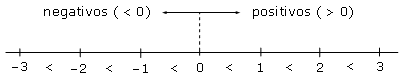
\includegraphics[width=4.2359in,height=0.8302in,keepaspectratio]{img/num18.png}
\end{center}


L’ordre en $\mathbb{R}$ pot també derivar-se a partir de la seva
representació gràfica com la recta real. D’aquesta manera, $a>b$
significa que el punt corresponent a $a$ es troba a la dreta del punt
corresponent a $b$, i $a<b$, significa que el punt corresponent a $a$
es troba a l’esquerra del punt corresponent a $b$.

Els ordres ja existents en els conjunts $\mathbb{Q},\mathbb{Z}$ i $%
\mathbb{N}$ són coherents amb l’ordre que acabem de definir en $%
\mathbb{R}$. Això vol dir, per exemple, que en considerar $\mathbb{Q}$
com subconjunt de $\mathbb{R}$, si $a,b$ són dos nombres racionals
tals que $a>b$ en $\mathbb{R}$, aleshores $a>b$ en $\mathbb{Q}$, és a dir,
l’ordre en $\mathbb{R}$ indueix sobre $\mathbb{Q}$ el mateix ordre que ja
coneixem en $\mathbb{Q}$.

\subsection{Enfocament algebraic}

Els dos enfocaments donats a l’apartat anterior són suficients per tenir
una idea clara de l’ordre en $\mathbb{R}$. Tanmateix, hi ha una forma de
expressar les relacions de desigualtat $>$ i $\geq$ que és especialment 
útil per fer les demostracions de les propietats de l’ordre en $%
\mathbb{R}$. Aquest nou enfocament no suposa cap intuïció prèvia (numèrica o geomètrica) sobre $\mathbb{R}$, només l’existència del
subconjunt dels nombres reals positius $\mathbb{R}^{+}$ i les
següents propietats:

\begin{enumerate}
\item Si $a,b\in \mathbb{R}^{+}$, aleshores $a+b\in \mathbb{R}^{+}$

\item Si $a,b\in \mathbb{R}^{+}$, aleshores $a\cdot b\in \mathbb{R}^{+}$

\item Si $a\in \mathbb{R}$, aleshores es compleix exactament una de les
següents relacions:%
\begin{equation*}
a\in \mathbb{R}^{+}\text{ \ \ \ \ \ \ }a=0\text{ \ \ \ \ \ \ }-a\in \mathbb{R%
}^{+}
\end{equation*}
\end{enumerate}

Les dues primeres propietats asseguren l’estabilitat sobre $\mathbb{R}^{+}$
de les operacions de suma i producte en $\mathbb{R}$. La tercera propietat
divideix $\mathbb{R}$ en tres tipus d’elements diferents; estableix que el
conjunt 
\begin{equation*}
\mathbb{R}^{-}=\{-a:a\in \mathbb{R}^{+}\}
\end{equation*}%
dels nombres reals negatius no té elements en comú amb $%
\mathbb{R}^{+}$ i, a més, que 
\begin{equation*}
\mathbb{R}=\mathbb{R}^{-}\cup \{0\}\cup \mathbb{R}^{+}
\end{equation*}%
A partir d’aquests supòsits (per altra banda, molt naturals), fem les
definicions següents:

\begin{enumerate}
\item Diem que $a$ és positiu i escrivim $a>0$, si $a\in \mathbb{R}%
^{+} $

\item Diem que $a$ és no negatiu i escrivim $a\geq 0$, si $a\in 
\mathbb{R}^{+}\cup \{0\}$

\item Diem que $a$ és negatiu i escrivim $a<0$, si $-a\in \mathbb{R}%
^{+}$

\item Diem que $a$ és no positiu i escrivim $a\leq 0$, si $-a\in 
\mathbb{R}^{+}\cup \{0\}$

\item Diem que $a$ és major que $b$ i escrivim $a>b$ o $b<a$, si $%
a-b\in \mathbb{R}^{+}$

\item Diem que $a$ és major o igual que $b$ i escrivim $a\geq b$ o $%
b\leq a$, si $a-b\in \mathbb{R}^{+}\cup \{0\}$
\end{enumerate}

\subsubsection{Propietats de l’ordre en $\mathbb{R}$}

Una de les utilitats pràctiques de les següents propietats és la seva
aplicació a la resolució d’inequacions. Per exemple, farem servir
aquestes propietats per resoldre una inequació com%
\begin{equation*}
-\frac{x}{3}+2<\frac{x}{2}+5
\end{equation*}%
En efecte, primer traiem els denominadors multiplicant cada membre per 
$6$. 
\begin{equation*}
-2x+12<3x+30
\end{equation*}%
observa que en multiplicar per un nombre real positiu el signe no se
invierte. Segon, 
\begin{align*}
-2x+12-3x &<&3x+30-3x \\
-5x+12 &<&30
\end{align*}%
observa que podem sumar qualsevol nombre real a ambdós membres
resultant una inequació equivalent. De la mateixa manera, tenim%
\begin{align*}
-5x+12-12 &<&30-12 \\
-5x &<&8
\end{align*}%
Tercer, multipliquem per $-1/5$ que, com que és negatiu, obligarà a
invertir el signe de la desigualtat. Així, obtenim%
\begin{equation*}
x>-\frac{8}{5}
\end{equation*}%
que ens diu que tots els nombres reals majors que $-8/5$ són solució de la inequació dada. Veurem en un altre apartat que les
solucions d’una inequació poden expressar-se mitjançant determinats
subconjunts de la recta real. En aquest cas, el conjunt de solucions se
expressaría com la següent semirecta abierta%
\begin{equation*}
\left( -\frac{8}{5},+\infty \right) 
\end{equation*}

\begin{enumerate}
\item \textbf{Propiedad transitiva}: per tot $a,b,c\in \mathbb{R}$, si $%
a>b$ i $b>c$, aleshores $a>c$
\end{enumerate}

En efecte, $a>b$ i $b>c$ si $a-b\in \mathbb{R}^{+}$ i $b-c\in \mathbb{R}^{+}$%
. Per tant,%
\begin{equation*}
(a-b)+(b-c)=a-c\in \mathbb{R}^{+}
\end{equation*}%
és a dir, $a>c$.

\begin{enumerate}
\item[2.] \textbf{Tricotomía}: donats dos nombres reals
qualssevol $a$ i $b$, es compleix una, i només una, d’aquestes tres
relacions%
\begin{equation*}
a>b\text{ \ \ \ \ \ \ }a=b\text{ \ \ \ \ \ \ }a<b
\end{equation*}
\end{enumerate}

En efecte, com $a-b\in \mathbb{R}$ aleshores es compleix exactament una de
les següents relacions:%
\begin{equation*}
a-b\in \mathbb{R}^{+}\text{ \ \ \ \ \ \ }a-b=0\text{ \ \ \ \ \ \ }%
-(a-b)=b-a\in \mathbb{R}^{+}
\end{equation*}%
és a dir,%
\begin{equation*}
a>b\text{ \ \ \ \ \ \ }a=b\text{ \ \ \ \ \ \ }b>a
\end{equation*}

\begin{enumerate}
\item[3.] \textbf{Propiedad reflexiva}: per tot $a\in \mathbb{R}$, $a\leq
a$.
\end{enumerate}

En efecte, $a-a=0\in \mathbb{R}^{+}\cup \{0\}$ i, per tant, $a\leq a$.

\begin{enumerate}
\item[4.] \textbf{Propiedad antisimétrica}: per tot $a,b\in \mathbb{R}$%
, si $a\geq b$ i $b\leq a$, aleshores $a=b$
\end{enumerate}

En efecte, suposem que fos $a\neq b$. Aleshores, per la propietat
anterior, es deduiría que $a>b$ o bé que $a<b$. Ara bé, no pot
passar $a>b$ perquè es contradiu amb la hipòtesi que $a\leq b$, ni
tampoc pot passar $a<b$ perquè es contradiu amb la hipòtesi que
\thinspace $a\geq b$. Per tant, no és possible que $a\neq b$ i, per
tant, ha de ser $a=b$.

\begin{enumerate}
\item[5.] \textbf{Propiedad de traslación}: si $a>b$, aleshores $a+c>b+c$%
, qualssevol que siguin $a,b,c\in \mathbb{R}$
\end{enumerate}

En efecte, $a>b$ si $a-b\in \mathbb{R}^{+}$. Podem escriure%
\begin{equation*}
a-b=(a+c)-(b+c)
\end{equation*}%
i, per tant,%
\begin{equation*}
(a+c)-(b+c)\in \mathbb{R}^{+}
\end{equation*}%
és a dir,%
\begin{equation*}
a+c>b+c
\end{equation*}%
Aquesta propietat s’expressa dient que el sentit d’una desigualtat%
\footnote{%
De la mateixa manera que amb el símbol $=$ expressem la relació de
igualtat, amb els símboels $>$ i $\geq$ expressaremos la relació
de desigualtat, que pot ser estricta en el primer cas, i no estricta, en
el segon.} no canvia si es suma un mateix nombre real a ambdós costats de
la desigualtat.

\begin{enumerate}
\item[6.] \textbf{Propiedad del producte per nombres positius}: si $a>b$
y $c>0$, aleshores $a\cdot c>b\cdot c$, qualssevol que siguin $a,b,c\in 
\mathbb{R}$
\end{enumerate}

En efecte, $a>b$ si $a-b\in \mathbb{R}^{+}$. Aleshores, com $c\in \mathbb{R}%
^{+}$, deduïm que%
\begin{equation*}
(a-b)\cdot c=a\cdot c-b\cdot c\in \mathbb{R}^{+}
\end{equation*}%
és a dir,%
\begin{equation*}
a\cdot c>b\cdot c
\end{equation*}%
Aquesta propietat es coneix dient que en multiplicar per un nombre
positiu ambdós costats d’una desigualtat, el sentit de la desigualtat no
canvia.

\begin{enumerate}
\item[7.] \textbf{Propiedad del producte per nombrés negatius}: si $a>b$
y $c<0$, aleshores $a\cdot c<b\cdot c$, qualssevol que siguin $a,b,c\in 
\mathbb{R}$
\end{enumerate}

En efecte, $a>b$ si $a-b\in \mathbb{R}^{+}$. Com $c<0$, aleshores $-c\in 
\mathbb{R}^{+}$ i, per tant,%
\begin{equation*}
(a-b)\cdot (-c)=b\cdot c-a\cdot c\in \mathbb{R}^{+}
\end{equation*}%
és a dir,%
\begin{equation*}
b\cdot c>a\cdot c
\end{equation*}%
Aquesta propietat es coneix dient que en multiplicar els dos membres de
una desigualtat per un nombre negatiu, el sentit de la desigualtat se
invierte.

\begin{enumerate}
\item[8.] \textbf{Propiedad de la suma}: si $a>b$ i $c>d$, aleshores $a+c>b+d$%
, qualssevol que siguin $a,b,c,d\in \mathbb{R}$
\end{enumerate}

En efecte, $a>b$ i $c>d$ si $a-b\in \mathbb{R}^{+}$ i $c-d\in \mathbb{R}^{+}$%
. Aleshores%
\begin{equation*}
(a-b)+(c-d)=(a+c)-(b+d)\in \mathbb{R}^{+}
\end{equation*}%
és a dir,%
\begin{equation*}
a+c>b+d
\end{equation*}

\subsection{Valor absolut}

Donat un nombre real qualsevol $a$, dels nombres $a$ i $-a$ el
major d’ells s’anomena \textbf{valor absolut} de $a$, i el designem per $%
\left\vert a\right\vert $. El valor absolut d’un nombre real pot
també definirse de la següent manera%
\begin{equation*}
\left\vert a\right\vert =\left\{ 
\begin{array}{ll}
a & \text{si }a\geq 0 \\ 
-a & \text{si }a<0%
\end{array}%
\right.
\end{equation*}%
és a dir, el valor absolut d’un nombre real no negatiu és el mateix nombre, mentre que si el nombre real és negatiu, el seu valor absolut
és l’oposat d’aquest nombre. En qualsevol cas, és evident que el
valor absolut d’un nombre real és sempre un nombre no negatiu.

\subsubsection{Propietats}

\begin{enumerate}
\item $\left\vert a\right\vert =0$ si i només si $a=0$
\end{enumerate}

En efecte, si $a=0$, aleshores $\left\vert 0\right\vert =0$. Recíprocamente, si fos $a\neq 0$, aleshores $-a\neq 0$ i, per tant, $%
\left\vert a\right\vert \neq 0$. Com a conseqüència, si $\left\vert
a\right\vert =0$, aleshores $a=0$.

Per exemple, si $\left\vert x-3\right\vert =0$, aleshores $x=3$.

\begin{enumerate}
\item[2.] $\left\vert -a\right\vert =\left\vert a\right\vert $, per tot $%
a\in \mathbb{R}$
\end{enumerate}

En efecte, si $a=0$, aleshores $\left\vert -0\right\vert =\left\vert
0\right\vert =0$. Si $a>0$, aleshores $-a<0$ i, per tant, $\left\vert
-a\right\vert =-(-a)=a=\left\vert a\right\vert $. Finalment, si $a<0$,
aleshores $-a>0$ i, per tant, $\left\vert -a\right\vert =-a=\left\vert
a\right\vert $.

Per exemple, si $\left\vert x-5\right\vert =2$, aleshores tenim dos
posibilidades: $x-5=2$ o $x-5=-2$, és a dir, $x=7$ o $x=3$.

\begin{enumerate}
\item[3.] $\left\vert a\cdot b\right\vert =\left\vert a\right\vert \cdot
\left\vert b\right\vert $, per tot $a,b\in \mathbb{R}$
\end{enumerate}

En efecte, si $a=0$ o $b=0$, aleshores $\left\vert a\cdot b\right\vert
=\left\vert a\right\vert \cdot \left\vert b\right\vert =0$. Si $a>0$ i $b>0$%
, aleshores $a\cdot b>0$ i, per tant, $\left\vert a\cdot b\right\vert
=a\cdot b=\left\vert a\right\vert \cdot \left\vert b\right\vert $. Si $a>0$
y $b<0$, aleshores $a\cdot b<0$ i, per tant,%
\begin{equation*}
\left\vert a\cdot b\right\vert =-(a\cdot b)=a\cdot (-b)=\left\vert
a\right\vert \cdot \left\vert b\right\vert
\end{equation*}%
De la mateixa manera es tracten els altres dos casos restants.

Per exemple, si $\left\vert (x-2)(x+5)\right\vert =0$, aleshores $\left\vert
x-2\right\vert \left\vert x+5\right\vert =0$. Per tant, $\left\vert
x-2\right\vert =0$ o $\left\vert x+5\right\vert =0$, d’on $x-2=0$ o $%
x+5=0$, és a dir, \thinspace $x=2$ o $x=-5$.

\begin{enumerate}
\item[4.] Si $b\geq 0$, aleshores $\left\vert a\right\vert \leq b$ si i només si $-b\leq a\leq b$
\end{enumerate}

En efecte, si $\left\vert a\right\vert \leq b$, aleshores per la definición de valor absolut es té $a\leq b$ i $-a\leq b$, però $-a\leq b$
equival a$ -b\leq a$. Recíprocamente, si $-b\leq a\leq b$, aleshores se
té $a\leq b$ com $-a\leq b$, ja que $b\geq 0$. Per tant, $\left\vert
a\right\vert \leq b$.

Per exemple, si $\left\vert x-2\right\vert \leq 3$, aleshores $-3\leq x-2\leq
3$, és a dir, $-3\leq x-2$ i $x-2\leq 3$. Per tant, $-1\leq x$ i $x\leq 5$.

\begin{enumerate}
\item[5.] $\left\vert a+b\right\vert \leq \left\vert a\right\vert
+\left\vert b\right\vert $, per tot $a,b\in \mathbb{R}$
\end{enumerate}

En efecte, puaixò que per definició $\left\vert a\right\vert \geq 0$ i $%
\left\vert b\right\vert \geq 0$, pel apartat anterior es té $%
-\left\vert a\right\vert \leq a\leq \left\vert a\right\vert$ i $-\left\vert
b\right\vert \leq b\leq \left\vert b\right\vert $. D’aquí, obtenim%
\begin{equation*}
a+b\leq \left\vert a\right\vert +\left\vert b\right\vert
\end{equation*}%
i%
\begin{equation*}
-(\left\vert a\right\vert +\left\vert b\right\vert )=-\left\vert
a\right\vert -\left\vert b\right\vert \leq a+b
\end{equation*}%
Per tant,%
\begin{equation*}
-(\left\vert a\right\vert +\left\vert b\right\vert )\leq a+b\leq \left\vert
a\right\vert +\left\vert b\right\vert
\end{equation*}%
i, en conseqüència,%
\begin{equation*}
\left\vert a+b\right\vert \leq \left\vert a\right\vert +\left\vert
b\right\vert
\end{equation*}

Per exemple, $2=\left\vert 2\right\vert =\left\vert (-3)+5\right\vert \leq
\left\vert -3\right\vert +\left\vert 5\right\vert =3+5=8$.

\subsection{Distància entre dos nombres reals}

Dos nombres reals qualssevol $a$ i $b$ corresponen amb dos punts 
$A$ i $B$ de la recta real. Aleshores, la longitud del segment $AB$ ve
donada per $\left\vert a-b\right\vert $. En efecte, suposem que $a<b$.
Aleshores poden donar-se els tres casos següents:

\begin{enumerate}
\item[a)] Que $0<a<b$, cas en què 
\begin{equation*}
\overline{AB}=\overline{OB}-\overline{OA}=b-a
\end{equation*}%

\begin{center}
  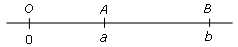
\includegraphics[width=2.5071in,height=0.5172in,keepaspectratio]{img/num25.png}
\end{center}
D’altra banda, com que és $a-b<0$, aleshores%
\begin{equation*}
\left\vert a-b\right\vert =-(a-b)=b-a
\end{equation*}%
i, per tant%
\begin{equation*}
\overline{AB}=\left\vert a-b\right\vert
\end{equation*}

\item[b)] Que $a<0<b$, cas en què 
\begin{equation*}
\overline{AB}=\overline{AO}+\overline{OB}=-a+b
\end{equation*}%

\begin{center}
  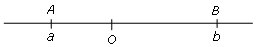
\includegraphics[width=2.7051in,height=0.5172in,keepaspectratio]{img/num44.png}
\end{center}
D’altra banda, com que és $b>0$, tenim que $-b<0$. De $a<0$ i $-b<0$%
, obtenim $a+(-b)=a-b<0$. Aleshores,%
\begin{equation*}
\left\vert a-b\right\vert =-(a-b)=-a+b
\end{equation*}%
i, per tant,%
\begin{equation*}
\overline{AB}=\left\vert a-b\right\vert
\end{equation*}

\item[c)] Que $a<b<0$, cas en què 
\begin{equation*}
\overline{AB}=\overline{AO}-\overline{BO}=-a-(-b)=-a+b
\end{equation*}%

\begin{center}
  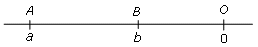
\includegraphics[width=2.7155in,height=0.5172in,keepaspectratio]{img/num45.png}
\end{center}
Per altra banda, com que és $a<b<0$, tenim que $a-b<0$. Aleshores,%
\begin{equation*}
\left\vert a-b\right\vert =-(a-b)=-a+b
\end{equation*}
\end{enumerate}

Definim la distància entre dos nombres reals $a$ i $b$ com la
longitud del segment $AB$. Segons el que acabem de demostrar, si
designem aquesta distància per $d(a,b)$, aleshores podem escriure%
\begin{equation*}
d(a,b)=\left\vert a-b\right\vert
\end{equation*}

Per exemple, 
\begin{equation*}
d(7,9)=\left\vert 7-9\right\vert =\left\vert -2\right\vert =2
\end{equation*}%
\begin{equation*}
d(-7,9)=\left\vert -7-9\right\vert =\left\vert -16\right\vert =16
\end{equation*}%
\begin{equation*}
d(-7,-9)=\left\vert -7-(-9)\right\vert =\left\vert 2\right\vert =2
\end{equation*}

\subsubsection{Propietats de la distància}

Les propietats de la distància són conseqüències immediates de les
propietats del valor absolut.

\begin{enumerate}
\item $d(a,b)\geq 0$, qualssevol que siguin $a,b\in \mathbb{R}$, i $d(a,b)=0$
si i només si $a=b$
\end{enumerate}

En efecte, com que és $d(a,b)=\left\vert a-b\right\vert$ és evident que $%
d(a,b)\geq 0$. A més, $d(a,b)=\left\vert a-b\right\vert =0$ si i només si $a-b=0$, és a dir, $a=b$.

\begin{enumerate}
\item[2.] $d(a,b)=d(b,a)$, qualssevol que siguin $a,b\in \mathbb{R}$
\end{enumerate}

En efecte, 
\begin{align*}
d(b,a) &=\left\vert b-a\right\vert \\
&=\left\vert -(a-b)\right\vert \\
&=\left\vert -1\right\vert \cdot \left\vert a-b\right\vert \\
&=\left\vert a-b\right\vert \\
&=d(a,b)
\end{align*}

\begin{enumerate}
\item[3.] $d(a,b)\leq d(a,c)+d(c,b)$, qualssevol que siguin $a,b,c\in 
\mathbb{R}$
\end{enumerate}

En efecte,%
\begin{align*}
d(a,b) &=\left\vert a-b\right\vert \\
&=\left\vert a-c+c-b\right\vert \\
&\leq &\left\vert a-c\right\vert +\left\vert c-b\right\vert \\
&=d(a,c)+d(c,b)
\end{align*}

\subsubsection{Entorns}

Si $a$ és un punt de la recta real (és a dir, qualsevol nombre real), i $%
r>0$, s’anomena \textbf{entorn de centre} $a$ \textbf{i radi} $r$ al
conjunt de punts la distància del qual a$a$ és menor que $r$. Si designem aquest
conjunt per $E_{r}(a)$, aleshores%
\begin{align*}
E_{r}(a) &=\{x\in \mathbb{R}:d(x,a)<r\} \\
&=\{x\in \mathbb{R}:\left\vert x-a\right\vert <r\}
\end{align*}%
És immediat comprovar que es compleix%
\begin{equation*}
E_{r}(a)=(a-r,a+r)
\end{equation*}%
D’això darrer es dedueix que la representació gràfica de l’
entorn $E_{r}(a)$ és com segueix:
\begin{center}
  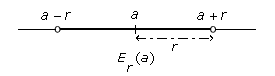
\includegraphics[width=2.8919in,height=0.8198in,keepaspectratio]{img/num51.png}
\end{center}
Si de l’entorn $E_{r}(a)$ es treu el
punt $a$, el conjunt que resulta s’anomena \textbf{entorn reduït de
centre} $a$ \textbf{i radi} $r$ i es denota per $E_{r}^{\ast }(a)$. Així%
, tenim%
\begin{equation*}
E_{r}^{\ast }(a)=E_{r}(a)-\{a\}
\end{equation*}

Per exemple, l’entorn de centre $2$ i radi $1/2$ serà el conjunt%
\begin{align*}
E_{1/2}(2) &=\{x\in \mathbb{R}:\left\vert x-\frac{1}{2}\right\vert <2\} \\
&=\left( 2-\frac{1}{2},2+\frac{1}{2}\right) \\
&=\left( \frac{3}{2},\frac{5}{2}\right)
\end{align*}

\subsection{Intervals i semirectes}

Recorda que hem utilitzat la paraula interval com a sinònim de
segment sobre la recta en definir un nombre real com a intersecció
d’una successió d’intervals encaixats. Amb la noció d’ordre ja
introduïda en $\mathbb{R}$, podem precisar encara més aquest concepte.

Si $a$ i $b$ són dos nombres reals amb $a\leq b$, aleshores el \textbf{%
interval obert} d’extrems $a$ i $b$ és el subconjunt de nombres
reals que designem per $(a,b)$ o bé per $]a,b[$ i que es defineix per%
\begin{equation*}
(a,b)=\{x\in \mathbb{R}:a<x<b\}
\end{equation*}%

\begin{center}
  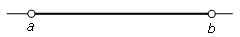
\includegraphics[width=2.5278in,height=0.4134in,keepaspectratio]{img/num46.png}
\end{center}
Si afegim els extrems al interval obert, s’obté el 
\textbf{interval tancat}, designat per $[a,b]$, i que es defineix per%
\begin{equation*}
\lbrack a,b]=\{x\in \mathbb{R}:a\leq x\leq b\}
\end{equation*}%

\begin{center}
  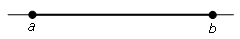
\includegraphics[width=2.5278in,height=0.4333in,keepaspectratio]{img/num47.png}
\end{center}
Si només afegim un dels extrems a l’interval obert,
s’obtenen els \textbf{intervals semioberts}:%
\begin{equation*}
\lbrack a,b)=\{x\in \mathbb{R}:a\leq x<b\}
\end{equation*}%

\begin{center}
  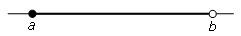
\includegraphics[width=2.5382in,height=0.403in,keepaspectratio]{img/num48.png}
\end{center}
%
\begin{equation*}
(a,b]=\{x\in \mathbb{R}:a<x\leq b\}
\end{equation*}%
En tots els casos, $a$ és l’extrem inferior de l’interval, $b$ és el
extrem superior i $b-a$ és la longitud de l’interval.

De la mateixa manera, si $a\in \mathbb{R}$, aleshores els subconjunts següents:%
\begin{equation*}
(a,+\infty )=\{x\in \mathbb{R}:x>a\}
\end{equation*}%
\begin{equation*}
(-\infty ,a)=\{x\in \mathbb{R}:x<a\}
\end{equation*}%

\begin{center}
  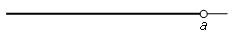
\includegraphics[width=2.4751in,height=0.3918in,keepaspectratio]{img/num49.png}
\end{center}
s’anomenen \textbf{semirectes obertes} d’extrem $a$. Si hi afegim l’extrem, obtenim%
\begin{equation*}
\lbrack a,+\infty )=\{x\in \mathbb{R}:x\geq a\}
\end{equation*}%
\begin{equation*}
(-\infty ,a]=\{x\in \mathbb{R}:x\leq a\}
\end{equation*}%

\begin{center}
  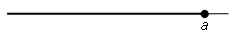
\includegraphics[width=2.4751in,height=0.403in,keepaspectratio]{img/num50.png}
\end{center}
les \textbf{semirectes tancades}. El símbol $\infty$ se
anomena \textbf{infinit} i no correspon amb cap nombre real;
en aquest context, en escriure $+\infty$ volem indicar una quantitat indeterminada
positiva tan gran com es vulgui, mentre que $-\infty$ indica una
quantitat indeterminada negativa tan petita com es vulgui.

\subsection{Conjunts fitats}

Sigui $A$ un subconjunt de $\mathbb{R}$. Diem que $k\in \mathbb{R}$ és una 
\textbf{cota superior} de $A$ si es compleix%
\begin{equation*}
x\leq k
\end{equation*}%
per a tot $x\in A$; diem que $k\in \mathbb{R}$ és una \textbf{cota
inferior} de $A$ si es compleix%
\begin{equation*}
k\leq x
\end{equation*}%
per a tot $x\in A$. Per exemple, en $\mathbb{R}^{+}$, qualsevol nombre
negatiu és cota inferior, i en $\mathbb{R}^{-}$, qualsevol nombre
positiu és cota superior. Diem que un subconjunt $A$ de $\mathbb{R}$ està \textbf{fitat superiorment} (resp. \textbf{inferiorment}) si $A$
té alguna cota superior (resp. inferior); diem que $A$ està 
\textbf{fitat} quan ho està superior i inferiorment. Per exemple,
qualsevol interval tancat $[a,b]$ és un conjunt fitat, ja que, $b$ es
cota superior i $a$ és cota inferior; la semirecta$(-\infty ,a)$ és un
conjunt que està fitat superiorment però no ho està
inferiorment.

Si $A$ és un subconjunt de $\mathbb{R}$ que està fitat superiorment
(resp. inferiorment), s’anomena \textbf{suprem} (resp. \textbf{ínfim}%
) de $A$, denotat per $\sup A$ (resp. $\inf A$), a la menor (resp. major)
de totes les cotes superiors (resp. inferiors); si el suprem (resp. ínfim) de $A$ és un element de $A$, aleshores el suprem (resp. ínfim)
s’anomena \textbf{màxim} (resp. \textbf{mínim}) de $A$ i se
designa per $\max A$ (resp. $\min A$).

Una propietat fonamental de $\mathbb{R}$ és la següent: Tot subconjunt
no buit fitat superiorment (resp. inferiorment) té suprem
(resp. ínfim).

\section{Potències enteres de nombres reals}

En aquesta secció donarem les propietats de les potències de nombres
reals amb exponent natural i veurem també com s’estén el
concepte formal de potència d’exponent natural al d’exponent enter.
Encara que no ho demostrarem, cal saber que les propietats donades per les
potències d’exponent natural s’estenen sense dificultat a les de
potències amb exponent enter.

\subsection{Potències d’exponent natural}

Si $a$ és un nombre real i $n$ és un nombre natural, s’anomena 
\textbf{potència }$n$\textbf{-èsima} de $a$, i la designem per $a^{n}$%
, al resultat de multiplicar $a$ per si mateix $n$ vegades, és a dir,%
\begin{equation*}
a^{n}=\overset{n\text{ vegades}}{\overbrace{a\cdot \cdots \cdot a}}
\end{equation*}%
En l’expressió $a^{n}$, el nombre $a$ s’anomena \textbf{base}, i $n$%
, \textbf{exponent}.

Per exemple,%
\begin{equation*}
\left( -\frac{1}{2}\right) ^{3}=\left( -\frac{1}{2}\right) \cdot \left( -%
\frac{1}{2}\right) \cdot \left( -\frac{1}{2}\right) =-\frac{1}{8}
\end{equation*}

\subsubsection{Propietats}

\begin{enumerate}
\item \textbf{Producte de potències}: el producte de potències de la mateixa
base és una altra potència de la mateixa base i d’exponent la suma dels
exponents, és a dir,%
\begin{equation*}
a^{n}\cdot a^{m}=a^{n+m}
\end{equation*}
\end{enumerate}

En efecte, 
\begin{align*}
a^{n}\cdot a^{m} &=\overset{n\text{ vegades}}{\overbrace{\left( a\cdot \cdots
\cdot a\right) }}\cdot \overset{m\text{ vegades}}{\overbrace{\left( a\cdot
\cdots \cdot a\right) }} \\
&=\overset{n+m\text{ vegades}}{\overbrace{a\cdot \cdots \cdot a}} \\
&=a^{n+m}
\end{align*}

Per exemple,%
\begin{equation*}
2^{3}\cdot 2^{2}=2^{3+2}=2^{5}
\end{equation*}

\begin{enumerate}
\item[2.] \textbf{Quocient de potències}: el quocient de potències de la
mateixa base és una altra potència de la mateixa base i d’exponent la diferència dels
exponents, és a dir,%
\begin{equation*}
\frac{a^{n}}{a^{m}}=a^{n-m}
\end{equation*}%
sempre que $a\neq 0$ i $n>m$.
\end{enumerate}

En efecte, suposant que $a\neq 0$ i $n>m$, tenim%
\begin{align*}
\frac{a^{n}}{a^{m}} &=\frac{\overset{n\text{ vegades}}{\overbrace{a\cdot
\cdots \cdot a}}}{\overset{m\text{ vegades}}{\overbrace{a\cdot \cdots \cdot a}}%
} \\
&=\frac{\overset{n-1\text{ vegades}}{\overbrace{a\cdot \cdots \cdot a}}}{%
\overset{m-1\text{ vegades}}{\overbrace{a\cdot \cdots \cdot a}}} \\
&&\vdots \\
&=\overset{n-m\text{ vegades}}{\overbrace{a\cdot \cdots \cdot a}} \\
&=a^{n-m}
\end{align*}%
Per exemple,%
\begin{align*}
\frac{3^{7}\cdot 3^{2}}{3^{5}} &=\frac{3^{7+2}}{3^{5}} \\
&=\frac{3^{9}}{3^{5}} \\
&=3^{4}
\end{align*}

En particular, si $m=n$, aleshores%
\begin{equation*}
\frac{a^{n}}{a^{n}}=1
\end{equation*}%
però, per altra banda, tenint present la propietat anterior, tenim%
\begin{equation*}
\frac{a^{n}}{a^{n}}=a^{n-n}=a^{0}
\end{equation*}%
Per tant, ha de ser 
\begin{equation*}
a^{0}=1
\end{equation*}%
sempre que $a\neq 0$.

\begin{enumerate}
\item[3.] \textbf{Potència d’una potència}: la potència d’una potència és
una altra potència de la mateixa base i d’exponent el producte dels exponents,
és a dir,%
\begin{equation*}
\left( a^{n}\right) ^{m}=a^{n\cdot m}
\end{equation*}
\end{enumerate}

En efecte,%
\begin{align*}
\left( a^{n}\right) ^{m} &=\overset{m\text{ vegades}}{\overbrace{a^{n}\cdot
\cdots \cdot a^{n}}} \\
&=a^{\overset{m\text{ vegades}}{\overbrace{n+\cdots +n}}} \\
&=a^{n\cdot m}
\end{align*}%
Per exemple,%
\begin{align*}
\left( \frac{2^{3}\cdot 2^{4}}{2^{5}}\right) ^{3} &=\left( \frac{2^{7}}{%
2^{5}}\right) ^{3} \\
&=\left( 2^{2}\right) ^{3} \\
&=2^{6}
\end{align*}

\begin{enumerate}
\item[4.] \textbf{Potència d’un producte}: la potència $n$-èsima d’un
producte és el producte de les potències $n$-èsimes dels factors, és a
dir,%
\begin{equation*}
\left( a\cdot b\right) ^{n}=a^{n}\cdot b^{n}
\end{equation*}
\end{enumerate}

En efecte,%
\begin{align*}
\left( a\cdot b\right) ^{n} &=\overset{n\text{ vegades}}{\overbrace{\left(
a\cdot b\right) \cdot \cdots \cdot \left( a\cdot b\right) }} \\
&=\overset{n\text{ vegades}}{\overbrace{\left( a\cdot \cdots \cdot a\right) }}%
\cdot \overset{n\text{ vegades}}{\overbrace{\left( b\cdot \cdots \cdot
b\right) }} \\
&=a^{n}\cdot b^{n}
\end{align*}%
En particular, tenim%
\begin{equation*}
(-a)^{n}=\left[ (-1)\cdot a\right] ^{n}=(-1)^{n}\cdot a^{n}=\left\{ 
\begin{array}{ll}
a^{n} & \text{si }n\text{ és par} \\ 
-a^{n} & \text{si }n\text{ és senar}%
\end{array}%
\right.
\end{equation*}%
Per exemple,%
\begin{align*}
\left[ (-2)^{3}\cdot 3^{2}\right] ^{4} &=\left[ (-2)^{3}\right] ^{4}\cdot
\left( 3^{2}\right) ^{4} \\
&=\left( -2\right) ^{12}\cdot 3^{8} \\
&=2^{12}\cdot 3^{8}
\end{align*}

\begin{enumerate}
\item[5.] \textbf{Potència d’un quocient}: la potència $n$-èsima d’un
quocient és el quocient de les potències $n$-èsimes del numerador i del
denominador, és a dir,%
\begin{equation*}
\left( \frac{a}{b}\right) ^{n}=\frac{a^{n}}{b^{n}}
\end{equation*}%
sempre que $b\neq 0$.
\end{enumerate}

En efecte,%
\begin{align*}
\left( \frac{a}{b}\right) ^{n} &=\overset{n\text{ vegades}}{\overbrace{\frac{a%
}{b}\cdot \cdots \cdot \frac{a}{b}}} \\
&=\frac{\overset{n\text{ vegades}}{\overbrace{\left( a\cdot \cdots \cdot
a\right) }}}{\overset{n\text{ vegades}}{\overbrace{\left( b\cdot \cdots \cdot
b\right) }}} \\
&=\frac{a^{n}}{b^{n}}
\end{align*}%
Per exemple,%
\begin{align*}
\left( \frac{2^{3}\cdot (-3)^{5}}{(-2)^{2}\cdot 3^{2}}\right) ^{4} &=\frac{%
\left[ 2^{3}\cdot (-3)^{5}\right] ^{4}}{\left[ (-2)^{2}\cdot 3^{2}\right]
^{4}} \\
&=\frac{\left( 2^{3}\right) ^{4}\cdot \left[ \left( -3\right) ^{5}\right]
^{4}}{\left[ \left( -2\right) ^{2}\right] ^{4}\cdot \left( 3^{2}\right) ^{4}}
\\
&=\frac{2^{12}\cdot \left( -3\right) ^{20}}{\left( -2\right) ^{8}\cdot 3^{8}%
} \\
&=\frac{2^{12}\cdot 3^{20}}{2^{8}\cdot 3^{8}} \\
&=2^{4}\cdot 3^{12}
\end{align*}

\subsection{Potències d’exponent enter}

Per estendre el concepte formal de potència d’exponent natural al de
exponent enter i negatiu, hem d’observar el fet següent:%
\begin{equation*}
a^{-n}=a^{0-n}=\frac{a^{0}}{a^{n}}=\frac{1}{a^{n}}
\end{equation*}%
on $n$ és un nombre natural i $a$ és un nombre real diferent de
zero. Aquest fet justifica la següent definició: si $n$ és un nombre natural i $a$ és un nombre real diferent de zero, s’anomena \textbf{%
potència d’exponent }$-n$ al nombre designat per $a^{-n}$ que es
defineix per%
\begin{equation*}
a^{-n}=\frac{1}{a^{n}}
\end{equation*}%
Com a conseqüència d’aquesta definició tenim que, si $n$ i $m$ són nombres naturals, aleshores%
\begin{equation*}
\frac{a^{n}}{a^{m}}=a^{n-m}
\end{equation*}%
fins i tot quan $m$ sigui major que $n$.

No és difícil demostrar que les propietats de les potències de
exponent natural són també vàlides per les potències de
exponent enter.

Per exemple,%
\begin{align*}
\frac{\left[ \left( \frac{2}{3}\right) ^{4}:\left( \frac{2}{3}\right) ^{3}%
\right] ^{-1}}{\left( \frac{2}{3}\right) ^{-2}} &=\frac{\left[ \left( \frac{%
2}{3}\right) ^{4}\right] ^{-1}:\left[ \left( \frac{2}{3}\right) ^{3}\right]
^{-1}}{\left( \frac{2}{3}\right) ^{-2}} \\
&=\frac{\left( \frac{2}{3}\right) ^{-4}:\left( \frac{2}{3}\right) ^{-3}}{%
\left( \frac{2}{3}\right) ^{-2}} \\
&=\frac{\left( \frac{2}{3}\right) ^{-4-(-3)}}{\left( \frac{2}{3}\right)
^{-2}} \\
&=\frac{\left( \frac{2}{3}\right) ^{-1}}{\left( \frac{2}{3}\right) ^{-2}} \\
&=\left( \frac{2}{3}\right) ^{-1-(-2)} \\
&=\frac{2}{3}
\end{align*}

Veurem en un altre apartat que, una vegada introduït el concepte d’arrel $%
n $-èsima, podrem estendre encara més el concepte de potència,
ampliant el camp de validesa de les propietats ja estudiades al de les
potències d’exponent racional.

\subsection{Notació científica}

Si la calculadora té la tecla $x^{y}$ podràs calcular potències
directament. Per exemple, per calcular $3^{5}$ has de teclejar%
\begin{equation*}
\begin{array}{ccccccccccc}
3 &  & x^{y} &  & 5 &  & = &  & \text{i obtindràs} &  & 243%
\end{array}%
\end{equation*}%
Tanmateix, quan els resultats de les potències són nombres en valor
absolut molt grans o molt petits les calculadores mostren els
resultats en notació científica. Per exemple, en calcular la
potència $100^{10}$%
\begin{equation*}
\begin{array}{ccccccccccc}
100 &  & x^{y} &  & 10 &  & = &  & \text{obtindràs} &  & 1~~^{20}%
\end{array}%
\end{equation*}%
que significa 
\begin{equation*}
1\times 10^{20}
\end{equation*}%
Un nombre en \textbf{notació científica} es representa com un
nombre comprès entre $1$ i $9$ multiplicat per una potència de $10$
amb exponent enter. En el camp de les ciències experimentals és molt
habitual expressar quantitats en notació científica. Per exemple,
el nombre de Avogadro 
\begin{equation*}
6.02\times 10^{23}
\end{equation*}%
o la massa del protó en grams%
\begin{equation*}
1.9\times 10^{-24}
\end{equation*}%
són dos nombres en notació científica que representen valors
aproximats dels valors reals de les magnituds mesurades en cada cas.
Observa que la potència de $10$ ens dona ràpidament una idea de l’ordre de
magnitud del nombre i el nombre de xifres amb què s’escriu el nombre correspon amb el grau de precisió que es vulgui donar a
la mesura. En general, utilitzarem aquesta notació per facilitar la
lectura i el maneig de nombres molt grans o molt petits en valor
absolut.

Si es vol introduir un nombre en notació científica en una
calculadora, farem servir la tecla EXP per introduir l’exponent de la potència.
Per exemple, $1.9\times 10^{-24}$ s’introdueix teclejant%
\begin{equation*}
\begin{array}{ccccccccccc}
1.9 &  & \text{EXP} &  & 24 &  & +/- &  & \text{i apareixerà} &  & 
1.9^{~-24}%
\end{array}%
\end{equation*}

\section{Arrels de nombres reals}

En la secció anterior hem après a calcular potències $n$-èsimes de
nombres reals i ara ens plantegem el problema invers: donat un nombre real $a$ volem trobar un altre, $x$, tal que la seva potència $n$-èsima sigui
igual a $a$, és a dir, volem resoldre l’equació%
\begin{equation*}
x^{n}=a
\end{equation*}%
En aquesta secció veurem que aquesta equació té sempre solució
si $a$ és no negatiu; les seves solucions s’obtenen a partir del càlcul
de l’arrel $n$-èsima de $a$ que es designa pel radical $\sqrt[n]{%
a}$. Veurem també que el problema invers queda resolt si limitem
l’atenció a les potències amb base un nombre real positiu $x$%
, verificant-se aleshores%
\begin{equation*}
\begin{array}{ccc}
\sqrt[n]{a}=x & \Longleftrightarrow & a=x^{n}%
\end{array}%
\end{equation*}%
En aquest cas, el càlcul invers de la potenciació s’anomena
radicació.%
\begin{equation*}
\begin{array}{ccc}
\sqrt[n]{a}=x & \overset{\text{Potenciació}}{\Longrightarrow } & a=x^{n}%
\end{array}%
\end{equation*}%
\begin{equation*}
\begin{array}{ccc}
\sqrt[n]{a}=x & \overset{\text{Radicació}}{\Longleftarrow } & a=x^{n}%
\end{array}%
\end{equation*}

\subsection{Arrels quadrades}

La diagonal d’un quadrat el costat del qual mesura una unitat de longitud és un nombre real positiu que satisfà l’equació%
\begin{equation*}
x^{2}=2
\end{equation*}%
Sabem que aquest nombre és irracional i, per tant, només podrem
escriure’l de forma aproximada perquè la seva expressió decimal té
infinites xifres decimals no periòdiques. Tot i que sigui impossible conèixer-lo
de forma exacta, sabem que hi ha mètodes per trobar el seu valor amb el
grau d’aproximació que es vulgui (mitjançant calculadora o per
aproximacions successives de nombres racionals o bé per l’algorisme clàssic d’extracció d’arrels quadrades). Tanmateix, podem
expressar-lo en forma exacta mitjançant el símbol del \textbf{radical} $%
\sqrt{~\ }$ per $\sqrt{2}$. L’expressió $\sqrt{2}$ s’anomena \textbf{arrel quadrada} de $2$. En escriure $\sqrt{2}$ ens referim al nombre
en la seva forma exacta, és a dir, al nombre que elevat al quadrat dona $2$,
és a dir,%
\begin{equation*}
\left( \sqrt{2}\right) ^{2}=2
\end{equation*}

Ara bé, l’equació $x^{2}=2$ té dues solucions: l’arrel
quadrada positiva, $\sqrt{2}$, i l’arrel quadrada negativa, $-\sqrt{2}$%
, ja que, es compleix%
\begin{align*}
\left( -\sqrt{2}\right) ^{2} &=\left( -\sqrt{2}\right) \cdot \left( -\sqrt{2%
}\right) \\
&=\left( \sqrt{2}\right) ^{2} \\
&=2
\end{align*}%
Observem que les equacions com, per exemple, $x^{2}=-1$ no tenen solució perquè el quadrat d’un nombre real mai és negatiu. Per
tant, les expressions $\sqrt{-1}$ i $-\sqrt{-1}$ no tenen sentit ja que
no representen cap nombre real.

En general, les equacions de la forma%
\begin{equation*}
x^{2}=a
\end{equation*}%
on $a$ és un nombre real positiu, tenen dues solucions: $\sqrt{a}
$ i $-\sqrt{a}$. Escrivim%
\begin{equation*}
\begin{array}{ccc}
x^{2}=a & \Longrightarrow & x=\pm \sqrt{a}%
\end{array}%
\end{equation*}

Exemples

\begin{enumerate}
\item $\sqrt{16}=4$ i $-\sqrt{16}=-4$, ja que $4^{2}=16$. Per tant, les
solucions de l’equació $x^{2}=16$ són $x=\pm 4$

\item Si $\sqrt{a}=13$, aleshores $a=13^{2}=169$

\item Si $-\sqrt{a}=-1.1$, aleshores $a=(1.1)^{2}=1.21$

\item Si $\sqrt{2x}=4$, aleshores $2x=4^{2}=16$ i, per tant, $x=8$

\item $\left( \sqrt{3}\right) ^{2}=3$ i $\left( \sqrt{5}\right) ^{3}=\left( 
\sqrt{5}\right) ^{2}\sqrt{5}=5\sqrt{5}$

\item $\left( 3\sqrt{7}\right) ^{2}=3^{2}\left( \sqrt{7}\right) ^{2}=9\cdot
7=63$

\item Si $\sqrt{2x-1}=5$, aleshores $2x-1=5^{2}=25$ i, per tant, $2x=26$ i,
en conseqüència, $x=13$
\end{enumerate}

\subsection{Arrels cúbiques}

L’aresta d’un cub el volum del qual és de tres unitats cúbiques és un nombre real positiu $x$ que satisfà l’equació%
\begin{equation*}
x^{3}=3
\end{equation*}%
Es pot demostrar que també és un nombre irracional i, per tant,
el seu valor numèric només podrà calcular-se de forma aproximada. Tanmateix, igual que abans, podem expressar-lo de forma exacta mitjançant el símbol del radical $\sqrt[3]{~~}$ per $\sqrt[3]{3}$. Aquesta expressió
s’anomena \textbf{arrel cúbica} de $3$, i amb ella ens referim al nombre que elevat al cub dona $3$, és a dir,%
\begin{equation*}
\left( \sqrt[3]{3}\right) ^{3}=3
\end{equation*}%
Ara, les equacions com, per exemple,%
\begin{equation*}
x^{3}=-8
\end{equation*}%
sí que tenen solució i, en aquest cas s’escriu com 
\begin{equation*}
x=\sqrt[3]{-8}=-2
\end{equation*}%
ja que%
\begin{equation*}
\left( -2\right) ^{3}=-8
\end{equation*}%
En general, l’equació 
\begin{equation*}
x^{3}=a
\end{equation*}%
on $a$ és qualsevol nombre real, té una única solució
que expressem com%
\begin{equation*}
x=\sqrt[3]{a}
\end{equation*}

\textbf{Exemples}:

\begin{enumerate}
\item $\sqrt[3]{-64}=-4$, ja que $(-4)^{3}=-64$

\item Si $\sqrt[3]{2x}=4$, aleshores $2x=4^{3}=64$ i, per tant, $x=32$

\item $\left( \sqrt[3]{5}\right) ^{3}=5$ i $\left( \sqrt[3]{3}\right)
^{4}=\left( \sqrt[3]{3}\right) ^{3}\sqrt[3]{3}=3\sqrt[3]{3}$

\item $\left( 2\sqrt[3]{5}\right) ^{3}=2^{3}\left( \sqrt[3]{5}\right)
^{3}=8\cdot 5=40$
\end{enumerate}

\subsection{Arrels enèsimes}

En general, podem trobar-nos amb equacions de la forma%
\begin{equation*}
x^{n}=a
\end{equation*}%
on $n$ és un nombre natural major que $1$ i $a\in \mathbb{R}$. Si $%
n$ és par i $a$ és positiu, l’equació admet dues solucions que s’
expressen en forma exacta mitjançant els radicals $\sqrt[n]{a}$ i $-\sqrt[n]{a}
$. Al radical $\sqrt[n]{a}$ s’anomena \textbf{arrel }$n$\textbf{-èsima positiva} de $a$, i a $-\sqrt[n]{a}$, \textbf{arrel }$n$\textbf{-%
èsima negativa} de $a$; $n$ s’anomena \textbf{índex }de l’arrel i $a$ s’anomena \textbf{radicand}. Amb aquestes expressions ens referim als
nombres reals la potència $n$-èsima dels quals és igual a $a$%
\begin{equation*}
\left( \sqrt[n]{a}\right) ^{n}=\left( -\sqrt[n]{a}\right) ^{n}=a
\end{equation*}%
Com hauràs observat tot d’una, els nombres reals negatius no
tenen arrels d’índex par. Si $n$ és senar i $a$ és qualsevol nombre real, l’equació admet una sola solució que s’expressa
per $\sqrt[n]{a}$; $\sqrt[n]{a}$ serà un nombre real negatiu si $a$
és negatiu, ja que com que és $n$ senar i es verifica que%
\begin{equation*}
\left( \sqrt[n]{a}\right) ^{n}=a
\end{equation*}%
aleshores $\left( \sqrt[n]{a}\right) ^{n}$ és negatiu i d’aquí, per
les regles dels signes, deduïm que $\sqrt[n]{a}$ ha de ser també
negatiu.

De la definició d’arrel $n$-èsima es dedueix en seguida la
següent propietat%
\begin{equation*}
\begin{array}{ccc}
\sqrt[n]{a}=x & \Longrightarrow & x^{n}=a%
\end{array}%
\end{equation*}%
En efecte, si $\sqrt[n]{a}=x$, aleshores%
\begin{equation*}
x^{n}=\left( \sqrt[n]{a}\right) ^{n}=a
\end{equation*}%
El recíproc d’aquesta propietat és fals, ja que, per exemple,%
\begin{equation*}
2^{2}=(-2)^{2}=4
\end{equation*}%
i, per tant, podríem escriure $\sqrt{4}=2$ i $\sqrt{4}=-2$, cosa que
no és possible ja que $-2\neq 2$. Aquesta contradicció es deu al fet que en efectuar potències d’exponent par, per les regles dels signes,
els nombres reals positius i negatius es confunden. Tanmateix, si
limitem l’atenció a les potències amb base un nombre real
positiu, aleshores es compleix el recíproc%
\begin{equation*}
\begin{array}{ccc}
\sqrt[n]{a}=x & \Longleftrightarrow & x^{n}=a%
\end{array}%
\end{equation*}%
En altres paraules, dir que $a$ és la potència $n$-èsima d’un nombre real positiu $x$ equival a dir que $x$ és l’arrel $n$-èsima de $a$. Hem definit així un procés de càlcul invers al de
la potenciació amb exponents naturals. Aquest procediment s’anomena \textbf{radicació} i consisteix a extreure l’arrel $n$-èsima d’un nombre positiu. El resultat d’efectuar aquest procés s’anomena arrel $n$-èsima d’aquest nombre.

\textbf{Exemples:}

\begin{enumerate}
\item $\sqrt{16}=4$, ja que $4^{2}=16$, però també $-\sqrt{16}=-4$, ja
que $(-4)^{2}=16$

\item $\sqrt[3]{27}=3$, ja que $3^{3}=27$

\item $\sqrt[5]{-32}=-2$ ja que $(-2)^{5}=-32$

\item $\sqrt{-16}$ no és un nombre real, ja que segons les regles dels
signes en la multiplicació dels nombres reals, no hi ha cap nombre real el quadrat del qual sigui negatiu

\item $\sqrt[3]{8a^{6}b^{3}}=2a^{2}b$, ja que $(2a^{2}b)^{3}=8a^{6}b^{3}$

\item $\sqrt{\frac{25a^{2}}{b^{4}}}=\frac{5a}{b^{2}}$, ja que $\left( \frac{%
5a}{b^{2}}\right) ^{2}=\frac{25a^{2}}{b^{4}}$
\end{enumerate}

\subsection{Càlcul d’arrels}

El càlcul d’arrels és immediat si es disposa de calculadora. El càlcul sense calculadora serà senzill si l’arrel és exacta,
ja que n’hi haurà prou amb efectuar la descomposició factorial del nombre i, després aplicar la definició d’arrel. Si l’arrel
no és exacta, sempre podrà aproximar-se per tempteig fins a un cert grau
mitjançant l’ús de les operacions elementals. Tanmateix, el mètode
per tempteig és llarg i pesat. En lloc seu, es fan servir algorismes de càlcul, com el que es coneix per extreure l’arrel quadrada d’un nombre, o també mètodes iteratius d’aproximació; en realitat,
les calculadores científiques tenen implementat un d’aquests
procediments iteratius perquè de forma automàtica calculi l’arrel de qualsevol índex. No tractarem de moment aquests darrers enfocaments de càlcul d’arrels.

\subsubsection{Algorisme per extreure arrels quadrades}

Si es disposa d’una calculadora amb la tecla $\sqrt{~~}$ el resultat és
immediat. Si no es disposa de calculadora, en els exemples que segueixen s’explica com s’extreu l’arrel quadrada d’un nombre pel
algorisme ordinari.

\begin{exemple}
Arrel quadrada de $73984$

Separem el nombre en blocs de dues xifres començant per les unitats i
es busca un nombre (en aquest cas és $2$) el quadrat del qual sigui menor o igual
que el primer bloc (en aquest cas és $7$). Ara es fa la resta
indicada, resultant $3$.
\begin{center}
  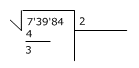
\includegraphics[width=1.4754in,height=0.736in,keepaspectratio]{img/num13.png}
\end{center}
D’aquesta manera hem obtingut la primera xifra de l’arrel.

Ara es baixa el bloc següent (en aquest cas és $39$) i es duplica el nombre trobat en el pas anterior (en aquest cas és $2\cdot 2=4\,$).
Aleshores es busca la xifra (en aquest cas és $7$) que, col·locada després
del doble del nombre trobat en el pas anterior formi un nombre
que multiplicat per aquesta xifra resulti un nombre menor o igual que el nombre que resulta després d’haver baixat el següent bloc (en
aquest cas $339$). Ara es fa la resta indicada, resultant $10$.%

\begin{center}
  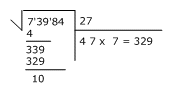
\includegraphics[width=1.8715in,height=0.9963in,keepaspectratio]{img/num14.png}
\end{center}
D’aquesta manera hem obtingut la següent xifra de l’arrel.

Es repeteix de nou aquest procés fins que no es puguin baixar més
blocs. Si l’última resta efectuada té com resultat $0$, l’arrel quadrada és exacta. En cas contrari, el valor de l’arrel serà un nombre decimal. En el nostre cas, obtenim que l’arrel
quadrada és exacta i el seu valor és $272$ com s’indica a continuació%

\begin{center}
  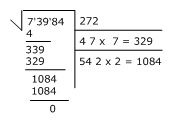
\includegraphics[width=1.8818in,height=1.3197in,keepaspectratio]{img/num15.png}
\end{center}


Podem comprovar el resultat mitjançant la calculadora, teclejant%
\begin{equation*}
\begin{array}{ccccccccc}
73984 &  & \sqrt{~~} &  & = &  & \text{i obtindràs} &  & 272%
\end{array}%
\end{equation*}
\end{exemple}

\begin{exemple}
Arrel quadrada de $123,45$ amb quatre xifres decimals

Separem el nombre en blocs de dues xifres començant per les unitats
(des de la coma) i es busca un nombre (en aquest cas és $1$) el quadrat del qual
sigui menor o igual que el primer bloc (en aquest cas és $1$). Ara s’efectua la resta indicada, resultant $0$.
\begin{center}
  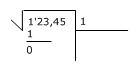
\includegraphics[width=1.465in,height=0.7567in,keepaspectratio]{img/num16.png}
\end{center}
D’aquesta manera hem obtingut la primera
xifra de l’arrel.

Ara es baixa el bloc següent (en aquest cas és $23$) i es duplica el nombre trobat en el pas anterior (en aquest cas és $2\cdot 1=2\,$).
Aleshores es busca la xifra (en aquest cas és $1$) que, col·locada després
del doble del nombre trobat en el pas anterior formi un nombre
que multiplicat per aquesta xifra resulti un nombre menor o igual que el nombre que resulta després d’haver baixat el següent bloc (en
aquest cas $23$). Ara es fa la resta indicada, resultant $2$.%

\begin{center}
  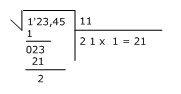
\includegraphics[width=1.913in,height=1.0066in,keepaspectratio]{img/num17.png}
\end{center}
D’aquesta manera hem obtingut la següent xifra de l’arrel.

En aquest cas, en baixar el bloc següent, ens trobem abans amb la coma.
Això vol dir que en el valor de l’arrel caldrà col·locar
també la coma. Aleshores, a partir de l’última xifra decimal del nombre caldrà afegir zeros fins a aconseguir que el nombre de
blocs de dues xifres a partir de la coma sigui el nombre de xifres
decimals amb el que volem trobar l’arrel. En aquest cas hi haurà
que afegir 6 zeros. A partir d’aquí, repetirem de nou el
procés fins que no es puguin baixar més blocs. 
\begin{center}
  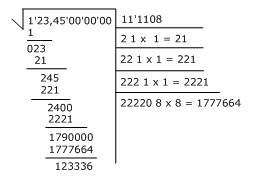
\includegraphics[width=2.6844in,height=1.9233in,keepaspectratio]{img/num19.png}
\end{center}
Observem que hi ha un pas en què
no hi ha cap xifra que, col·locada després del doble del nombre
trobat en el pas anterior (en aquest cas és $2222)$ formi un nombre
que sigui menor o igual que el nombre que resulta després d’haver
baixat el següent bloc (en aquest cas és $17900$). Aleshores es baixarà
el següent bloc i es col·locarà $0$ com la següent xifra decimal de
l’arrel.

Podem comprovar el resultat mitjançant la calculadora, teclejant%
\begin{equation*}
\begin{array}{ccccccccc}
123.45 &  & \sqrt{~~} &  & = &  & \text{i obtindràs} &  & 11.11080555%
\end{array}%
\end{equation*}%
la seva aproximació per defecte amb quatre xifres decimals coincideix amb el nostre resultat.
\end{exemple}

\subsubsection{Càlcul d’arrels amb calculadora}

Si la calculadora té la tecla amb la funció $x^{1/y}$, per calcular 
$\sqrt[3]{3796416}$ has de teclejar%
\begin{equation*}
\begin{array}{ccccccccccc}
3796416 &  & x^{1/y} &  & 3 &  & = &  & \text{i obtindràs} &  & 156%
\end{array}%
\end{equation*}%
De la mateixa manera, per calcular $\sqrt[5]{217.4}$ has de teclejar 
\begin{equation*}
\begin{array}{ccccccccccc}
217.4 &  & x^{1/y} &  & 5 &  & = &  & \text{i obtindràs} &  & 2.933944593%
\end{array}%
\end{equation*}%
Si no té la tecla $x^{1/y}$ però sí té la tecla per la potència$%
x^{y}$, també podem calcular les arrels anteriors de la
següent manera%
\begin{equation*}
\begin{array}{ccccccccccc}
3796416 &  & x^{y} &  & 3 &  & 1/x &  & = &  & 156%
\end{array}%
\end{equation*}%
\begin{equation*}
\begin{array}{ccccccccccc}
217.4 &  & x^{y} &  & 5 &  & 1/x &  & = &  & 2.933944593%
\end{array}%
\end{equation*}

\subsubsection{Càlcul d’arrels exactes per descomposició}

Per exemple, per calcular $\sqrt[3]{3796416}$ per descomposició,
primer descomponem el radicand en factors primers
\begin{center}
  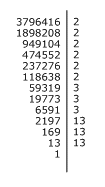
\includegraphics[width=1.1217in,height=1.977in,keepaspectratio]{img/num20.png}
\end{center}
resultant%
\begin{equation*}
3796416=2^{6}\cdot 3^{3}\cdot 13^{3}
\end{equation*}%
Ara bé, per les propietats de les potències, podem escriure també%
\begin{align*}
3796416 &=(2^{2}\cdot 3\cdot 13)^{3} \\
&=156^{3}
\end{align*}%
Per tant, tenim%
\begin{equation*}
\sqrt[3]{3796416}=\sqrt[3]{156^{3}}=156
\end{equation*}%
De la mateixa manera, per calcular $\sqrt{0.0064}$, primer observem que 
\begin{equation*}
0.0064=64\cdot 10^{-4}=2^{6}\cdot 10^{-4}=(2^{3}\cdot 10^{-2})^{2}
\end{equation*}%
i, per tant,%
\begin{equation*}
\sqrt{0.0064}=2^{3}\cdot 10^{-2}=0.08
\end{equation*}

\subsubsection{Càlcul d’arrels per tempteig}

Per calcular per tempteig una arrel com, per exemple, $\sqrt[3]{5.23}$,
primer observem que%
\begin{equation*}
1<\sqrt[3]{5.23}<2
\end{equation*}%
pues%
\begin{equation*}
1^{3}=1<5.23<8=2^{3}
\end{equation*}%
D’aquesta manera, sabem que 
\begin{equation*}
\sqrt[3]{5.23}=1.\cdots
\end{equation*}%
Ara, trobaremos la xifra de les dècimes també per tempteig.
Observa els càlculs següents:%
\begin{equation*}
\begin{array}{c}
1.5^{3}=3.375<5.23 \\ 
1.6^{3}=4.096<5.23 \\ 
1.7^{3}=4.913<5.23 \\ 
1.8^{3}=5.832>5.23%
\end{array}%
\end{equation*}%
A partir d’aquí, és clar que%
\begin{equation*}
1.7<\sqrt[3]{5.23}<1.8
\end{equation*}%
i, per tant, sabem que 
\begin{equation*}
\sqrt[3]{5.23}=1.7~\cdots
\end{equation*}%
De la mateixa manera es trobaran les altres xifres decimals. Així,
per les centesimas tenim%
\begin{equation*}
\begin{array}{c}
1.75^{3}=5.359375>5.23 \\ 
1.74^{3}=5.268024>5.23 \\ 
1.73^{3}=5.177717<5.23%
\end{array}%
\end{equation*}%
i, per tant, obtenim que 
\begin{equation*}
\sqrt[3]{5.23}=1.73~\cdots
\end{equation*}

\section{Càlcul amb radicals}

En el càlcul amb arrels o amb expressions que les contenen es
poden aplicar les propietats usuals de les operacions amb nombres
reals i certes propietats que veurem en aquest apartat. Al càlcul
fet d’aquesta manera, sense utilitzar valors aproximats dels nombres
irracionals que apareixen (és a dir, expressant-los en forma exacta, com a
radicals), s’anomena habitualment \textbf{càlcul amb radicals}.

Les propietats de les operacions amb radicals són:

\begin{enumerate}
\item Producte%
\begin{equation*}
\sqrt[n]{a}\cdot \sqrt[n]{b}=\sqrt[n]{a\cdot b}
\end{equation*}

\item Potència%
\begin{equation*}
\left( \sqrt[n]{a}\right) ^{m}=\sqrt[n]{a^{m}}
\end{equation*}

\item Quocient%
\begin{equation*}
\frac{\sqrt[n]{a}}{\sqrt[n]{b}}=\sqrt[n]{\frac{a}{b}}
\end{equation*}

\item Radicació%
\begin{equation*}
\sqrt[n]{\sqrt[m]{a}}=\sqrt[nm]{a}
\end{equation*}
\end{enumerate}

A més, pel càlcul amb radicals,serà convenient conèixer
les següents tècniques:

\begin{enumerate}
\item Obtenció de radicals semblants%
\begin{equation*}
\sqrt[mn]{a^{m}}=\sqrt[n]{a}
\end{equation*}

\item Simplificació de radicals%
\begin{equation*}
\sqrt[n]{a^{pn+q}\cdot b}=a^{p}\cdot \sqrt[n]{a^{q}\cdot b}
\end{equation*}

\item Suma i resta de radicals

\item Racionalització de denominadors
\end{enumerate}

\subsection{Propietats de les operacions amb arrels}

Per provar les propietats següents utilitzarem les propietats de les
potències d’exponent natural, la definició d’arrel $n$-èsima
segons la qual $\sqrt[n]{a}=b$ si $b^{n}=a$ i la propietat fonamental%
\begin{equation*}
\left( \sqrt[n]{a}\right) ^{n}=a
\end{equation*}%
sempre que l’arrel tingui sentit.

\subsubsection{Arrel d’un producte}

Aquesta propietat s’expressa dient que l’arrel d’un producte és igual
al producte de les arrels. En termes més formales: per tot $%
a,b\in \mathbb{R}$ i per tot $n\in \mathbb{N}$ es compleix%
\begin{equation*}
\sqrt[n]{a\cdot b}=\sqrt[n]{a}\cdot \sqrt[n]{b}
\end{equation*}%
sempre que les tres arrels tinguin sentit.

En efecte,%
\begin{align*}
\left( \sqrt[n]{a}\cdot \sqrt[n]{b}\right) ^{n} &=\left( \sqrt[n]{a}\right)
^{n}\cdot \left( \sqrt[n]{b}\right) ^{n} \\
&=a\cdot b
\end{align*}%
Per la propietat associativa de la multiplicació, aquesta propietat pot
estendre’s a més de dos factors. Per exemple, per tres factors,
tenim%
\begin{align*}
\sqrt[n]{a\cdot b\cdot c} &=\sqrt[n]{a\cdot \left( b\cdot c\right) } \\
&=\sqrt[n]{a}\cdot \sqrt[n]{b\cdot c} \\
&=\sqrt[n]{a}\cdot \left( \sqrt[n]{b}\cdot \sqrt[n]{c}\right) \\
&=\sqrt[n]{a}\cdot \sqrt[n]{b}\cdot \sqrt[n]{c}
\end{align*}

\textbf{Exemples}:

\begin{enumerate}
\item 
\begin{align*}
\sqrt[4]{32a^{4}}\cdot \sqrt[4]{2a^{2}}\cdot \sqrt[4]{4a^{2}} &=\sqrt[4]{%
32a^{4}\cdot 2a^{2}\cdot 4a^{2}} \\
&=\sqrt[4]{256a^{8}} \\
&=\sqrt[4]{2^{8}a^{8}} \\
&=\sqrt[4]{\left( 2a\right) ^{8}} \\
&=(2a)^{2} \\
&=4a^{2}
\end{align*}

\item 
\begin{align*}
\left( 2\sqrt{5}-\sqrt{3}\right) ^{2} &=\left( 2\sqrt{5}\right) ^{2}-2\cdot
2\sqrt{5}\cdot \sqrt{3}+\left( \sqrt{3}\right) ^{2} \\
&=4\sqrt{5^{2}}-4\sqrt{15}+\sqrt{3^{2}} \\
&=20-4\sqrt{15}+3 \\
&=23-4\sqrt{15}
\end{align*}
\end{enumerate}

\subsubsection{Potència d’una arrel}

De la propietat del producte d’arrels s’obté de forma immediata la
propietat de la potència d’una arrel que s’expressa dient que la
potència d’una arrel és l’arrel de la potència, és a dir,%
\begin{equation*}
\left( \sqrt[n]{a}\right) ^{m}=\sqrt[n]{a^{m}}
\end{equation*}%
sempre que les dues arrels tinguin sentit.

En efecte,%
\begin{align*}
\left( \sqrt[n]{a}\right) ^{m} &=\overset{m\text{ factors}}{\overbrace{%
\sqrt[n]{a}\cdot \cdots \cdot \sqrt[n]{a}}} \\
&=\sqrt[n]{\overset{m\text{ factors}}{\overbrace{a\cdot \cdots \cdot a}}}
\\
&=\sqrt[n]{a^{m}}
\end{align*}

\textbf{Exemples}:

\begin{enumerate}
\item 
\begin{align*}
\left( \sqrt[4]{729}\right) ^{2} &=\left( \sqrt[4]{3^{6}}\right) ^{2} \\
&=\sqrt[4]{\left( 3^{6}\right) ^{2}} \\
&=\sqrt[4]{3^{12}} \\
&=3^{3}=27
\end{align*}

\item 
\begin{align*}
\left( \sqrt[3]{9a^{2}b}\right) ^{2}\left( \sqrt[3]{3ab^{2}}\right) ^{2} &=%
\sqrt[3]{\left( 9a^{2}b\right) ^{2}}\sqrt[3]{\left( 3ab^{2}\right) ^{2}} \\
&=\sqrt[3]{81a^{4}b^{2}}\sqrt[3]{9a^{2}b^{4}} \\
&=\sqrt[3]{\left( 81a^{4}b^{2}\right) \left( 9a^{2}b^{4}\right) } \\
&=\sqrt[3]{729a^{6}b^{6}} \\
&=\sqrt[3]{\left( 3ab\right) ^{6}} \\
&=\left( 3ab\right) ^{2}=9a^{2}b^{2}
\end{align*}
\end{enumerate}

\subsubsection{Arrel d’un quocient}

Aquesta propietat s’expressa dient que l’arrel d’un quocient és igual
al quocient de les arrels. En terme més formales: per tot $%
a,b\in \mathbb{R}$ amb $b\neq 0$ i per tot $n\in \mathbb{N}$ es compleix%
\begin{equation*}
\sqrt[n]{\frac{a}{b}}=\frac{\sqrt[n]{a}}{\sqrt[n]{b}}
\end{equation*}%
sempre que les tres arrels tinguin sentit.

En efecte,%
\begin{align*}
\left( \frac{\sqrt[n]{a}}{\sqrt[n]{b}}\right) ^{n} &=\frac{\left( \sqrt[n]{a%
}\right) ^{n}}{\left( \sqrt[n]{b}\right) ^{n}} \\
&=\frac{a}{b}
\end{align*}

\textbf{Exemples}:

\begin{enumerate}
\item 
\begin{align*}
\frac{\sqrt[4]{8x^{2}y}}{\sqrt[4]{2xy^{2}}} &=\sqrt[4]{\frac{8x^{2}y}{%
2xy^{2}}} \\
&=\sqrt[4]{\frac{4x}{y}}
\end{align*}

\item 
\begin{align*}
\frac{\sqrt[3]{3a}\sqrt[3]{9a^{4}}}{\sqrt[3]{3a^{2}}} &=\frac{\sqrt[3]{%
\left( 3a\right) \left( 9a^{4}\right) }}{\sqrt[3]{3a^{2}}} \\
&=\frac{\sqrt[3]{27a^{5}}}{\sqrt[3]{3a^{2}}} \\
&=\sqrt[3]{\frac{27a^{5}}{3a^{2}}} \\
&=\sqrt[3]{9a^{3}} \\
&=\sqrt[3]{9}\sqrt[3]{a^{3}} \\
&=a\sqrt[3]{9}
\end{align*}
\end{enumerate}

\subsubsection{Arrel d’una arrel}

Aquesta propietat s’expressa afirmant que l’arrel d’una arrel és
una altra arrel que té com a índex el producte dels índexs de
les arrels, és a dir, 
\begin{equation*}
\sqrt[n]{\sqrt[m]{a}}=\sqrt[nm]{a}
\end{equation*}%
sempre que les tres arrels tinguin sentit.

En efecte, 
\begin{align*}
\left( \sqrt[n]{\sqrt[m]{a}}\right) ^{nm} &=\left[ \left( \sqrt[n]{\sqrt[m]{%
a}}\right) ^{n}\right] ^{m} \\
&=\left( \sqrt[m]{a}\right) ^{m} \\
&=a
\end{align*}

\textbf{Exemples}:

\begin{enumerate}
\item 
\begin{equation*}
\frac{\sqrt[3]{\sqrt{ab}}}{\sqrt{\sqrt[3]{ab}}}=\frac{\sqrt[6]{ab}}{\sqrt[6]{%
ab}}=1
\end{equation*}

\item 
\begin{align*}
\left( \sqrt[4]{\sqrt[3]{729}}\right) ^{3} &=\left( \sqrt[12]{729}\right)
^{3} \\
&=\left( \sqrt[12]{3^{6}}\right) ^{3} \\
&=\sqrt[12]{\left( 3^{6}\right) ^{3}} \\
&=\sqrt[12]{3^{18}} \\
&=\sqrt[12]{3^{12}\cdot 3^{6}} \\
&=\sqrt[12]{3^{12}}\sqrt[12]{3^{6}} \\
&=3\sqrt[12]{3^{6}} \\
&=3\sqrt{3}
\end{align*}
\end{enumerate}

\subsection{Radicals equivalents}

Observa que es compleix%
\begin{equation*}
3=\sqrt{9}=\sqrt[3]{27}=\sqrt[4]{81}
\end{equation*}%
és a dir, el nombre $3$ està representat per diferents radicals.
Es diu aleshores que aquests radicals són equivalents. Dos radicals s’
anomenen \textbf{equivalents} quan tenen les mateixes arrels.

Per obtenir un radical equivalent a un de donat tenim la següent propietat%
\begin{equation*}
\sqrt[mn]{a^{m}}=\sqrt[n]{a}
\end{equation*}%
En efecte,%
\begin{align*}
\left( \sqrt[mn]{a^{m}}\right) ^{n} &=\sqrt[mn]{\left( a^{m}\right) ^{n}} \\
&=\sqrt[mn]{a^{mn}} \\
&=a
\end{align*}%
Amb aquesta propietat, veiem que 
\begin{equation*}
\sqrt[3]{2^{2}}=\sqrt[6]{2^{4}}=\sqrt[9]{2^{6}}=\sqrt[12]{2^{8}}=\sqrt[15]{%
2^{10}}
\end{equation*}%
i, en general, aquesta propietat permetrà simplificar radicals,
reduir-los a índex comú i comparar-los.

\textbf{Exemples}:

\begin{itemize}
\item \textbf{Simplificació de radicals:}%
\begin{align*}
\sqrt[4]{a^{12}\sqrt[4]{b^{24}}} &=\sqrt[4]{a^{12}}\cdot \sqrt[4]{\sqrt[4]{%
b^{24}}} \\
&=\sqrt[3]{a^{3}}\cdot \sqrt[16]{b^{24}} \\
&=a\sqrt{b^{3}} \\
&=a\sqrt{b^{2}}\sqrt{b} \\
&=ab\sqrt{b}
\end{align*}

\item \textbf{Reducció de radicals a índex comú:} tota
multiplicació i divisió amb radicals de diferents índexs
pot transformar-se de manera que tots els radicals tinguin el mateix índex. Una vegada feta aquesta transformació, efectuarem les operacions
segons les propietats de les arrels.

\begin{enumerate}
\item 
\begin{align*}
\frac{\sqrt[6]{2/3}}{\sqrt[3]{3/2}} &=\frac{\sqrt[6]{2/3}}{\sqrt[6]{\left(
3/2\right) ^{2}}} \\
&=\frac{\sqrt[6]{2/3}}{\sqrt[6]{9/4}} \\
&=\sqrt[6]{\frac{2/3}{9/4}} \\
&=\sqrt[6]{\frac{8}{27}} \\
&=\sqrt[6]{\frac{2^{3}}{3^{3}}} \\
&=\sqrt[6]{\left( \frac{2}{3}\right) ^{3}} \\
&=\sqrt{\frac{2}{3}}
\end{align*}

\item 
\begin{align*}
\frac{\sqrt{ab}\sqrt{a\sqrt{b}}}{\sqrt{a\sqrt[3]{b}}} &=\frac{\sqrt{ab}%
\left( \sqrt{a}\sqrt{\sqrt{b}}\right) }{\sqrt{a}\sqrt{\sqrt[3]{b}}} \\
&=\frac{\sqrt{ab}\sqrt{a}\sqrt[4]{b}}{\sqrt{a}\sqrt[6]{b}} \\
&=\frac{\sqrt[12]{\left( ab\right) ^{6}}\sqrt[12]{a^{6}}\sqrt[12]{b^{3}}}{%
\sqrt[12]{a^{6}}\sqrt[12]{b^{2}}} \\
&=\frac{\sqrt[12]{a^{12}b^{9}}}{\sqrt[12]{a^{6}b^{2}}} \\
&=\sqrt[12]{\frac{a^{12}b^{9}}{a^{6}b^{2}}} \\
&=\sqrt[12]{a^{6}b^{7}} \\
&=\sqrt[12]{a^{6}}\sqrt[12]{b^{7}} \\
&=\sqrt{a}\sqrt[12]{b^{7}}
\end{align*}
\end{enumerate}

\item \textbf{Comparació de radicals:} Ordenar de menor a major els
següents radicals%
\begin{equation*}
\sqrt[4]{5},\sqrt[6]{3^{4}},\sqrt[8]{7^{5}}
\end{equation*}%
reduint-los a índex comú i sabent que $mcm(4,6,8)=24$,
obtenim%
\begin{equation*}
\sqrt[24]{5^{6}},\sqrt[24]{\left( 3^{4}\right) ^{4}},\sqrt[24]{\left(
7^{5}\right) ^{3}}
\end{equation*}%
és a dir,%
\begin{equation*}
\sqrt[24]{5^{6}},\sqrt[24]{3^{16}},\sqrt[24]{7^{15}}
\end{equation*}%
Per tant,%
\begin{equation*}
\sqrt[4]{5}=\sqrt[24]{5^{6}}<\sqrt[6]{3^{4}}=\sqrt[24]{3^{16}}<\sqrt[8]{7^{5}%
}=\sqrt[24]{7^{15}}
\end{equation*}%
doncs, una vegada reduïts els radicals a índex comú, estem en
condicions de comparar-los i ordenar-los: és major el radical que té
radicand més gran.
\end{itemize}

\subsection{Introducció i extracció de factors en una arrel}

La formulació d’aquesta propietat ve donada per%
\begin{equation*}
\sqrt[n]{a^{n}\cdot b}=a\sqrt[n]{b}
\end{equation*}%
sempre que les arrels tinguin sentit. Llegint d’esquerra a dreta,
es fa la \textbf{extracció} d’un factor de l’arrel i, de
dreta a esquerra, es realitza la \textbf{introducció} d’un factor en
l’arrel. En efecte,%
\begin{align*}
\left( a\sqrt[n]{b}\right) ^{n} &=a^{n}\left( \sqrt[n]{b}\right) ^{n} \\
&=a^{n}\cdot b
\end{align*}%
Podem donar una formulació més general d’aquesta propietat
escribiendo que%
\begin{equation*}
\sqrt[n]{a^{pn+q}\cdot b}=a^{p}\cdot \sqrt[n]{a^{q}\cdot b}
\end{equation*}%
En efecte,%
\begin{align*}
\left( a^{p}\cdot \sqrt[n]{a^{q}\cdot b}\right) ^{n} &=a^{pn}\cdot \left( 
\sqrt[n]{a^{q}\cdot b}\right) ^{n} \\
&=a^{pn}\cdot \left( a^{q}\cdot b\right) \\
&=a^{pn+q}\cdot b
\end{align*}

\textbf{Exemples}:

\begin{itemize}
\item Extracció:

\begin{enumerate}
\item 
\begin{align*}
\sqrt[3]{a^{7}} &=\sqrt[3]{a^{2\cdot 3+1}} \\
&=a^{2}\sqrt[3]{a}
\end{align*}

\item 
\begin{align*}
\sqrt[4]{a^{6}b^{8}c^{12}} &=\sqrt[4]{a^{1\cdot 4+2}}\sqrt[4]{b^{2\cdot 4}}%
\sqrt[4]{c^{3\cdot 4}} \\
&=a\sqrt[4]{a^{2}}b^{2}c^{3} \\
&=ab^{2}c^{3}\sqrt{a}
\end{align*}
\end{enumerate}

\item Introducció:

\begin{enumerate}
\item 
\begin{align*}
2\cdot \sqrt[5]{3}\cdot 6\cdot \sqrt[7]{5} &=2\cdot \sqrt[35]{3^{7}}\cdot
6\cdot \sqrt[35]{5^{5}} \\
&=\sqrt[35]{2^{35}}\cdot \sqrt[35]{3^{7}}\cdot \sqrt[35]{6^{35}}\cdot \sqrt[%
35]{5^{5}} \\
&=\sqrt[35]{2^{35}\cdot 3^{7}\cdot 6^{35}\cdot 5^{5}}
\end{align*}

\item 
\begin{align*}
\frac{1}{2}a^{3}b\sqrt{\frac{b^{5}}{a^{4}}} &=\sqrt{\frac{\left(
a^{3}b\right) ^{2}b^{5}}{2^{2}a^{4}}} \\
&=\sqrt{\frac{a^{6}b^{7}}{4a^{4}}} \\
&=\sqrt{\frac{a^{2}b^{7}}{4}}
\end{align*}
\end{enumerate}
\end{itemize}

\subsection{Suma d’arrels}

És important assenyalar que l’arrel d’una suma no és la suma de les
arrels%
\begin{equation*}
\sqrt[n]{a+b}\neq \sqrt[n]{a}+\sqrt[n]{b}
\end{equation*}%
Per provar aquest fet, donem l’exemple següent%
\begin{equation*}
\sqrt{9}=\sqrt{2+7}\neq \sqrt{2}+\sqrt{7}
\end{equation*}%
ja que%
\begin{align*}
\left( \sqrt{2}+\sqrt{7}\right) ^{2} &=\left( \sqrt{2}\right) ^{2}+2\sqrt{2}%
\sqrt{7}+\left( \sqrt{7}\right) ^{2} \\
&=9+2\sqrt{14}\neq 9
\end{align*}%
En general, quan hi hagi una suma d’arrels només podrem
agrupar els radicals semblants, utilitzant la propietat distributiva de la
multiplicació respecte de la suma%
\begin{equation*}
b\sqrt[n]{a}+c\sqrt[n]{a}=(b+c)\sqrt[n]{a}
\end{equation*}

\textbf{Exemples}:

\begin{enumerate}
\item 
\begin{align*}
\sqrt{45}-2\sqrt[3]{81}-3\sqrt{180}+\sqrt[3]{375}-\sqrt{80} &=\sqrt{5\cdot
3^{2}}-2\sqrt[3]{3^{3+1}}-3\sqrt{2^{2}\cdot 3^{2}\cdot 5}+\sqrt[3]{%
5^{3}\cdot 3}-\sqrt{2^{2\cdot 2}\cdot 5} \\
&=3\sqrt{5}-2\cdot 3\sqrt[3]{3}-3\cdot 2\cdot 3\sqrt{5}+5\sqrt[3]{3}-2^{2}%
\sqrt{5} \\
&=(3-18-4)\sqrt{5}+(5-6)\sqrt[3]{3} \\
&=-19\sqrt{5}-\sqrt[3]{3}
\end{align*}

\item 
\begin{align*}
5\sqrt[3]{a^{2}b}-3\sqrt[3]{a^{2}b}+7\sqrt[3]{a^{2}b} &=(5-3+7)\sqrt[3]{%
a^{2}b} \\
&=9\sqrt[3]{a^{2}b}
\end{align*}
\end{enumerate}

\subsection{Racionalització de denominadors}

La fracció%
\begin{equation*}
\frac{3\sqrt{2}+1}{5\sqrt{2}+\sqrt{3}}
\end{equation*}%
en tenir denominador irracional, es considera poc
adequada si volem efectuar la divisió indicada. Amb l’objectiu d’evitar errors en els càlculs —ja que caldria usar aproximacions
racionals tant en el numerador com en el denominador, i intentar treballar
tant com sigui possible amb valors exactes, es recomana en aquests casos
fer abans la racionalització del denominador. La \textbf{%
racionalització de denominadors} és una tècnica que consisteix a
transformar la fracció dada, de denominador irracional, en una altra
fracció equivalent però amb denominador racional. La tècnica general
consistirà a trobar una expressió que en multiplicar-la pel
numerador i el denominador de la fracció s’aconsegueixi que en el
denominador de la nova fracció equivalent no aparegui cap arrel.

Estudiarem dos casos:

\begin{cas}
si el denominador conté una sola arrel, la fracció és del tipus%
\begin{equation*}
\frac{a}{c\sqrt[n]{b^{m}}}
\end{equation*}%
on $m$ és menor que $n$. La racionalització s’aconsegueix
multiplicant numerador i denominador per%
\begin{equation*}
\sqrt[n]{b^{n-m}}
\end{equation*}
\end{cas}

En efecte,%
\begin{equation*}
\frac{a}{c\sqrt[n]{b^{m}}}=\frac{a}{c\sqrt[n]{b^{m}}}\cdot \frac{\sqrt[n]{%
b^{n-m}}}{\sqrt[n]{b^{n-m}}}=\frac{a\sqrt[n]{b^{n-m}}}{c\sqrt[n]{b^{n}}}=%
\frac{a\sqrt[n]{b^{n-m}}}{cb}
\end{equation*}%
Si fos $m$ major que $n$, es podria extreure fora del radical una
certa potència de $b$ i dins quedaria una potència de $b$ de
exponent més petit que $n$ i a partir d’aquí es procediria igual que abans.

\textbf{Exemples}:

\begin{enumerate}
\item 
\begin{align*}
\frac{5}{\sqrt[3]{16}} &=\frac{5}{\sqrt[3]{2^{4}}} \\
&=\frac{5}{2\sqrt[3]{2}} \\
&=\frac{5}{2\sqrt[3]{2}}\cdot \frac{\sqrt[3]{2^{2}}}{\sqrt[3]{2^{2}}} \\
&=\frac{5\sqrt[3]{4}}{2\sqrt[3]{2^{3}}} \\
&=\frac{5\sqrt[3]{4}}{4}
\end{align*}

\item 
\begin{align*}
\frac{3}{4\sqrt{5}} &=\frac{3}{4\sqrt{5}}\cdot \frac{\sqrt{5}}{\sqrt{5}} \\
&=\frac{3\sqrt{5}}{4\sqrt{5^{2}}} \\
&=\frac{3\sqrt{5}}{20}
\end{align*}
\end{enumerate}

\begin{cas}
Si el denominador conté una suma o diferència d’arrels quadrades,
la fracció és del tipus%
\begin{equation*}
\frac{a}{b\sqrt{c}\pm d\sqrt{e}}
\end{equation*}%
La racionalització s’aconsegueix multiplicant numerador i denominador per
l’expressió conjugada del denominador $b\sqrt{c}\mp d\sqrt{e}$
\end{cas}

En efecte, tenint present que%
\begin{align*}
\left( b\sqrt{c}+d\sqrt{e}\right) \left( b\sqrt{c}-d\sqrt{e}\right)
&=\left( b\sqrt{c}\right) ^{2}-\left( d\sqrt{e}\right) ^{2} \\
&=b^{2}\left( \sqrt{c}\right) ^{2}-d^{2}\left( \sqrt{e}\right) ^{2} \\
&=b^{2}c-d^{2}e
\end{align*}%
aleshores tenim%
\begin{align*}
\frac{a}{b\sqrt{c}+d\sqrt{e}} &=\frac{a}{b\sqrt{c}+d\sqrt{e}}\cdot \frac{b%
\sqrt{c}-d\sqrt{e}}{b\sqrt{c}-d\sqrt{e}} \\
&=\frac{a\left( b\sqrt{c}-d\sqrt{e}\right) }{b^{2}c-d^{2}e} \\
&=\frac{ab\sqrt{c}-ad\sqrt{e}}{b^{2}c-d^{2}e}
\end{align*}%
i de forma anàloga es fa l’altre cas.

\textbf{Exemples}:

\begin{enumerate}
\item 
\begin{align*}
\frac{5}{5-\sqrt{5}} &=\frac{5}{5-\sqrt{5}}\cdot \frac{5+\sqrt{5}}{5+\sqrt{5%
}} \\
&=\frac{5\left( 5+\sqrt{5}\right) }{5^{2}-\left( \sqrt{5}\right) ^{2}} \\
&=\frac{5\left( 5+\sqrt{5}\right) }{20} \\
&=\frac{5+\sqrt{5}}{4}
\end{align*}

\item 
\begin{align*}
\frac{3\sqrt{2}+1}{5\sqrt{2}+\sqrt{3}} &=\frac{3\sqrt{2}+1}{5\sqrt{2}+\sqrt{%
3}}\cdot \frac{5\sqrt{2}-\sqrt{3}}{5\sqrt{2}-\sqrt{3}} \\
&=\frac{\left( 3\sqrt{2}+1\right) \left( 5\sqrt{2}-\sqrt{3}\right) }{\left(
5\sqrt{2}\right) ^{2}-\left( \sqrt{3}\right) ^{2}} \\
&=\frac{15\left( \sqrt{2}\right) ^{2}-3\sqrt{2}\sqrt{3}+5\sqrt{2}-\sqrt{3}}{%
5^{2}\left( \sqrt{2}\right) ^{2}-3} \\
&=\frac{30-3\sqrt{6}+5\sqrt{2}-\sqrt{3}}{47}
\end{align*}
\end{enumerate}

\subsection{Potències d’exponent racional}

En prendre el conveni de definir $a^{-n}$ per%
\begin{equation}
a^{-n}=\frac{1}{a^{n}}  \label{eq:potencia-exponent-negatiu}
\end{equation}%
amb $a>0$ i $n\in \mathbb{N}$, es va poder estendre el càlcul de potències
d’exponent natural al d’exponent enter. Amb la finalitat d’ampliar encara més el concepte formal de potència, ara prenem el conveni de definir $%
a^{m/n}$ per%
\begin{equation*}
a^{m/n}=\sqrt[n]{a^{m}}
\end{equation*}%
amb $n,m\in \mathbb{N}$ i $a\geq 0$, i d’acord amb (\ref{eq:potencia-exponent-negatiu}), convenim també definir $a^{-m/n}$ per%
\begin{equation*}
a^{-m/n}=\frac{1}{a^{m/n}}=\frac{1}{\sqrt[n]{a^{m}}}
\end{equation*}%
amb $n,m\in \mathbb{N}$ i $a>0$. D’aquesta manera, podem estendre el càlcul de potències al d’exponent racional, ja que qualsevol nombre
racional pot escriure’s com $m/n$, on $m\in \mathbb{Z}$ i $n\in 
\mathbb{N}$. A més, aquest conveni és coherent amb la teoria ja
coneguda, és a dir, que totes les propietats que coneixem per les
potències d’exponent enter continuen sent vàlides per les
potències d’exponent racional.

\textbf{Exemples}:

\begin{enumerate}
\item $32^{3/5}=8$, ja que $\sqrt[5]{32^{3}}=\sqrt[5]{(2^{5})^{3}}=\sqrt[5]{%
2^{15}}=2^{3}=8$.

\item $81^{-1/4}=1/3$, ja que $\sqrt[4]{81^{-1}}=\sqrt[4]{1/81}=\sqrt[4]{%
1/3^{4}}=1/\sqrt[4]{3^{4}}=1/3$.
\end{enumerate}

\subsubsection{Propietats de les potències d’exponent racional}

Aquestes propietats són importants perquè quan hàgim d’operar amb
expressions en les que apareguin exponents racionals, podrem usar-les
directament sense necessitat de transformar-les en radicals.

Tanmateix, el següent exemple mostra dues maneres de calcular una expressió amb exponents racionals: una, consisteix a utilitzar les propietats
de les potències d’exponent racional, i l’altra, consisteix a transformar
primer l’expressió en una altra equivalent amb radicals i després
utilitzar les propietats dels radicals.

\begin{equation*}
\frac{3^{1/3}\cdot 3^{1/2}}{3^{2/5}}=\frac{3^{\frac{1}{3}+\frac{1}{2}}}{3^{%
\frac{2}{5}}}=3^{\frac{1}{3}+\frac{1}{2}-\frac{2}{5}}=3^{\frac{13}{30}}
\end{equation*}%
\begin{align*}
\frac{3^{1/3}\cdot 3^{1/2}}{3^{2/5}} &=\frac{\sqrt[3]{3}\cdot \sqrt{3}}{%
\sqrt[5]{3^{2}}} \\
&=\frac{\sqrt[6]{3^{2}}\cdot \sqrt[6]{3^{3}}}{\sqrt[5]{3^{2}}} \\
&=\frac{\sqrt[6]{3^{5}}}{\sqrt[5]{3^{2}}} \\
&=\frac{\sqrt[30]{3^{25}}}{\sqrt[30]{3^{12}}} \\
&=\sqrt[30]{3^{13}}
\end{align*}

\textbf{Producte de potències}: Per tot $a>0$, $m,r\in \mathbb{Z}$ i $%
n,s\in \mathbb{N}$, es compleix%
\begin{equation*}
a^{\frac{m}{n}}\cdot a^{\frac{r}{s}}=a^{\frac{m}{n}+\frac{r}{s}}
\end{equation*}%
En efecte,%
\begin{align*}
a^{\frac{m}{n}}\cdot a^{\frac{r}{s}} &=\sqrt[n]{a^{m}}\cdot \sqrt[s]{a^{r}}
\\
&=\sqrt[ns]{a^{ms}}\cdot \sqrt[ns]{a^{nr}} \\
&=\sqrt[ns]{a^{ms}\cdot a^{nr}} \\
&=\sqrt[ns]{a^{ms+nr}} \\
&=a^{\frac{ms+nr}{ns}} \\
&=a^{\frac{m}{n}+\frac{r}{s}}
\end{align*}

\textbf{Exemples}:

\begin{enumerate}
\item[1.] 
\begin{align*}
3^{1/2}\cdot 3^{1/3}\cdot 3^{1/6} &=\left( 3^{1/2}\cdot 3^{1/3}\right)
\cdot 3^{1/6} \\
&=3^{\frac{1}{2}+\frac{1}{3}}\cdot 3^{\frac{1}{6}} \\
&=3^{\left( \frac{1}{2}+\frac{1}{3}\right) +\frac{1}{6}} \\
&=3^{\frac{1}{2}+\frac{1}{3}+\frac{1}{6}} \\
&=3^{1}=3
\end{align*}

\item[2.] 
\begin{align*}
a^{1/2}\cdot b\cdot a^{3}\cdot b^{-1/3} &=\left( a^{1/2}\cdot b\right)
\cdot \left( a^{3}\cdot b^{-1/3}\right) \\
&=\left( a^{1/2}\cdot b\right) \cdot \left( b^{-1/3}\cdot a^{3}\right) \\
&=a^{1/2}\cdot \left( b\cdot b^{-1/3}\right) \cdot a^{3} \\
&=a^{1/2}\cdot \left( b^{1-\frac{1}{3}}\cdot a^{3}\right) \\
&=a^{1/2}\cdot \left( a^{3}\cdot b^{2/3}\right) \\
&=\left( a^{1/2}\cdot a^{3}\right) \cdot b^{2/3} \\
&=a^{\frac{1}{2}+3}\cdot b^{2/3} \\
&=a^{7/2}\cdot b^{2/3}
\end{align*}
\end{enumerate}

\textbf{Quocient de potències}: Per tot $a>0$, $m,r\in \mathbb{Z}$ i $%
n,s\in \mathbb{N}$, es compleix%
\begin{equation*}
\frac{a^{\frac{m}{n}}}{a^{\frac{r}{s}}}=a^{\frac{m}{n}-\frac{r}{s}}
\end{equation*}%
En efecte,%
\begin{align*}
\frac{a^{\frac{m}{n}}}{a^{\frac{r}{s}}} &=\frac{\sqrt[n]{a^{m}}}{\sqrt[s]{%
a^{r}}} \\
&=\frac{\sqrt[ns]{a^{ms}}}{\sqrt[ns]{a^{nr}}} \\
&=\sqrt[ns]{\frac{a^{ms}}{a^{nr}}} \\
&=\sqrt[ns]{a^{ms-nr}} \\
&=a^{\frac{ms-nr}{ns}} \\
&=a^{\frac{m}{n}-\frac{r}{s}}
\end{align*}

\textbf{Exemples}:

\begin{enumerate}
\item 
\begin{align*}
\frac{5^{3}\cdot \left( \frac{1}{5}\right) ^{2}\cdot 5^{3/4}}{5^{4}\cdot
\left( \frac{1}{5}\right) ^{3}} &=\frac{5^{3}\cdot 5^{-2}\cdot 5^{3/4}}{%
5^{4}\cdot 5^{-3}} \\
&=\frac{\left( 5^{3}\cdot 5^{-2}\right) \cdot 5^{3/4}}{5} \\
&=\frac{5\cdot 5^{3/4}}{5} \\
&=5^{3/4}
\end{align*}

\item 
\begin{align*}
\frac{a^{2}b^{-1}a^{3/2}b^{4}}{a^{-1/2}b^{-2}a^{1/3}} &=\frac{\left(
a^{2}b^{-1}\right) \left( a^{3/2}b^{4}\right) }{a^{-1/2}\left(
b^{-2}a^{1/3}\right) } \\
&=\frac{\left( a^{2}b^{-1}\right) \left( b^{4}a^{3/2}\right) }{%
a^{-1/2}\left( a^{1/3}b^{-2}\right) } \\
&=\frac{a^{2}\left( b^{-1}b^{4}\right) a^{3/2}}{\left(
a^{-1/2}a^{1/3}\right) b^{-2}} \\
&=\frac{a^{2}\left( b^{3}a^{3/2}\right) }{a^{-1/6}b^{-2}} \\
&=\frac{a^{2}\left( a^{3/2}b^{3}\right) }{a^{-1/6}b^{-2}} \\
&=\frac{\left( a^{2}a^{3/2}\right) b^{3}}{a^{-1/6}b^{-2}} \\
&=\frac{a^{7/2}b^{3}}{a^{-1/6}b^{-2}} \\
&=\frac{a^{7/2}}{a^{-1/6}}\cdot \frac{b^{3}}{b^{-2}} \\
&=a^{22/6}\cdot b^{5} \\
&=a^{11/3}\cdot b^{5}
\end{align*}
\end{enumerate}

\textbf{Potència d’una potència}: Per tot $a>0$, $m,r\in \mathbb{Z}$ i $%
n,s\in \mathbb{N}$, es compleix%
\begin{equation*}
\left( a^{\frac{m}{n}}\right) ^{\frac{r}{s}}=a^{\frac{m}{n}\cdot \frac{r}{s}}
\end{equation*}%
En efecte,%
\begin{align*}
\left( a^{\frac{m}{n}}\right) ^{\frac{r}{s}} &=\left( \sqrt[n]{a^{m}}%
\right) ^{\frac{r}{s}} \\
&=\sqrt[s]{\left( \sqrt[n]{a^{m}}\right) ^{r}} \\
&=\sqrt[s]{\sqrt[n]{\left( a^{m}\right) ^{r}}} \\
&=\sqrt[ns]{a^{mr}} \\
&=a^{\frac{mr}{ns}} \\
&=a^{\frac{m}{n}\cdot \frac{r}{s}}
\end{align*}

\textbf{Exemples}:

\begin{enumerate}
\item 
\begin{align*}
\left( 2^{1/2}\right) ^{1/3}\cdot \left( 2^{4}\right) ^{1/5} &=2^{1/6}\cdot
2^{4/5} \\
&=2^{29/30}
\end{align*}

\item 
\begin{align*}
\frac{\left( a^{1/2}\cdot \frac{a^{1/3}}{a^{2/5}}\right) ^{1/4}}{a^{-2/3}}
&=\frac{\left( a^{1/2}\cdot a^{-1/15}\right) ^{1/4}}{a^{-2/3}} \\
&=\frac{a^{1/8}\cdot a^{-1/60}}{a^{-2/3}} \\
&=\frac{a^{13/120}}{a^{-2/3}} \\
&=a^{31/40}
\end{align*}
\end{enumerate}

\textbf{Potència d’un producte}: Per tot $a,b>0$, $m\in \mathbb{Z}$ i $%
n\in \mathbb{N}$, es compleix%
\begin{equation*}
(a\cdot b)^{m/n}=a^{m/n}\cdot b^{m/n}
\end{equation*}%
En efecte,%
\begin{align*}
(a\cdot b)^{m/n} &=\sqrt[n]{(a\cdot b)^{m}} \\
&=\sqrt[n]{a^{m}\cdot b^{m}} \\
&=\sqrt[n]{a^{m}}\cdot \sqrt[n]{b^{m}} \\
&=a^{n/m}\cdot b^{n/m}
\end{align*}

\textbf{Exemples}:

\begin{enumerate}
\item 
\begin{align*}
\left( \frac{3}{4}\right) ^{3/2}\cdot 2^{3/2}\cdot \left( \frac{2}{3}\right)
^{3/2} &=\left[ \left( \frac{3}{4}\right) ^{3/2}\cdot 2^{3/2}\right] \cdot
\left( \frac{2}{3}\right) ^{3/2} \\
&=\left( \frac{3}{4}\cdot 2\right) ^{3/2}\cdot \left( \frac{2}{3}\right)
^{3/2} \\
&=\left( \frac{3}{2}\right) ^{3/2}\cdot \left( \frac{2}{3}\right) ^{3/2} \\
&=\left( \frac{3}{2}\cdot \frac{2}{3}\right) ^{3/2} \\
&=1^{3/2}=\sqrt{1^{3}}=1
\end{align*}

\item 
\begin{align*}
\left( a^{3}\cdot b^{-4}\right) ^{5/6} &=\left( a^{3}\right) ^{5/6}\cdot
\left( b^{-4}\right) ^{5/6} \\
&=a^{5/2}\cdot b^{-10/3}
\end{align*}
\end{enumerate}

\textbf{Potència d’un quocient}: Per tot $a,b>0$, $m\in \mathbb{Z}$ i $%
n\in \mathbb{N}$, es compleix%
\begin{equation*}
\left( \frac{a}{b}\right) ^{m/n}=\frac{a^{m/n}}{b^{m/n}}
\end{equation*}%
En efecte,%
\begin{align*}
\left( \frac{a}{b}\right) ^{m/n} &=\sqrt[n]{\left( \frac{a}{b}\right) ^{m}}
\\
&=\sqrt[n]{\frac{a^{m}}{b^{m}}} \\
&=\frac{\sqrt[n]{a^{m}}}{\sqrt[n]{b^{m}}} \\
&=\frac{a^{m/n}}{b^{m/n}}
\end{align*}

\textbf{Exemples}:

\begin{enumerate}
\item 
\begin{align*}
\frac{(16\cdot 9\cdot 25)^{1/3}}{\left( 8\cdot 27\cdot 5\right) ^{1/3}}
&=\left( \frac{16\cdot 9\cdot 25}{8\cdot 27\cdot 5}\right) ^{1/3} \\
&=\left( \frac{10}{3}\right) ^{1/3}
\end{align*}

\item 
\begin{align*}
\left( \frac{a^{2}b}{b^{1/2}a}\right) ^{3}\cdot \left( \frac{a^{-1/3}b^{5}}{%
a^{2}b^{3}}\right) ^{1/2} &=\frac{\left( a^{2}b\right) ^{3}}{\left(
b^{1/2}a\right) ^{3}}\cdot \frac{\left( a^{-1/3}b^{5}\right) ^{1/2}}{\left(
a^{2}b^{3}\right) ^{1/2}} \\
&=\frac{a^{6}b^{3}}{b^{3/2}a^{3}}\cdot \frac{a^{-1/6}b^{5/2}}{ab^{3/2}} \\
&=\frac{a^{35/6}b^{11/2}}{a^{4}b^{3}} \\
&=a^{11/6}\cdot b^{5/2}
\end{align*}
\end{enumerate} 